\documentclass[12pt,twoside]{report}
\usepackage{lmodern}
\usepackage{amssymb,amsmath}
\usepackage{ifxetex,ifluatex}
\usepackage{fixltx2e} % provides \textsubscript
\ifnum 0\ifxetex 1\fi\ifluatex 1\fi=0 % if pdftex
  \usepackage[T1]{fontenc}
  \usepackage[utf8]{inputenc}
\else % if luatex or xelatex
  \ifxetex
    \usepackage{mathspec}
    \usepackage{xltxtra,xunicode}
  \else
    \usepackage{fontspec}
  \fi
  \defaultfontfeatures{Mapping=tex-text,Scale=MatchLowercase}
  \newcommand{\euro}{€}
\fi
% use upquote if available, for straight quotes in verbatim environments
\IfFileExists{upquote.sty}{\usepackage{upquote}}{}
% use microtype if available
\IfFileExists{microtype.sty}{%
\usepackage{microtype}
\UseMicrotypeSet[protrusion]{basicmath} % disable protrusion for tt fonts
}{}
\usepackage[margin=1in]{geometry}
\usepackage{graphicx}
\makeatletter
\def\maxwidth{\ifdim\Gin@nat@width>\linewidth\linewidth\else\Gin@nat@width\fi}
\def\maxheight{\ifdim\Gin@nat@height>\textheight\textheight\else\Gin@nat@height\fi}
\makeatother
% Scale images if necessary, so that they will not overflow the page
% margins by default, and it is still possible to overwrite the defaults
% using explicit options in \includegraphics[width, height, ...]{}
\setkeys{Gin}{width=\maxwidth,height=\maxheight,keepaspectratio}
\ifxetex
  \usepackage[setpagesize=false, % page size defined by xetex
              unicode=false, % unicode breaks when used with xetex
              xetex]{hyperref}
\else
  \usepackage[unicode=true]{hyperref}
\fi
\hypersetup{breaklinks=true,
            bookmarks=true,
            pdfauthor={},
            pdftitle={},
            colorlinks=true,
            citecolor=blue,
            urlcolor=blue,
            linkcolor=magenta,
            pdfborder={0 0 0}}
\urlstyle{same}  % don't use monospace font for urls
\setlength{\parindent}{0pt}
\setlength{\parskip}{6pt plus 2pt minus 1pt}
\setlength{\emergencystretch}{3em}  % prevent overfull lines
\setcounter{secnumdepth}{0}

%%% Use protect on footnotes to avoid problems with footnotes in titles
\let\rmarkdownfootnote\footnote%
\def\footnote{\protect\rmarkdownfootnote}

%%% Change title format to be more compact
\usepackage{titling}

% Create subtitle command for use in maketitle
\newcommand{\subtitle}[1]{
  \posttitle{
    \begin{center}\large#1\end{center}
    }
}

\setlength{\droptitle}{-2em}
  \title{}
  \pretitle{\vspace{\droptitle}}
  \posttitle{}
  \author{}
  \preauthor{}\postauthor{}
  \date{}
  \predate{}\postdate{}

\usepackage[english,brazilian]{babel} % suporte para línguas
\usepackage[utf8]{inputenc} % codificação

\usepackage{subfig, epsfig}
\captionsetup[subfigure]{style=default, 
  margin=0pt, parskip=0pt, hangindent=0pt, indention=0pt, 
  singlelinecheck=true, labelformat=parens, labelsep=space}

\usepackage{ae}
\usepackage{aecompl}
\usepackage{booktabs}
\usepackage[T1] {fontenc}

\usepackage{footnote}

% Notas criadas nas tabelas ficam no fim das tabelas
\makesavenoteenv{tabular}

\usepackage{fancyhdr}

\fancypagestyle{plain}
{
  \fancyhf{}%
  \renewcommand{\headrulewidth}{0pt}%
  \fancyfoot[C]{\thepage}
}

\usepackage{graphicx,wrapfig} % para incluir figuras
\usepackage[all]{xy} % para incluir diagramas
\usepackage{amsfonts, amssymb, amsthm, amsmath, amscd, textcomp} % pacote AMS
\usepackage{color, float, bbm, multicol, rotating}
\usepackage{verbatim, listings, booktabs}

\usepackage{caption} % Customizar as legendas de figuras e tabelas
\usepackage{array} % Elementos extras para formatação de tabelas

\usepackage[switch,pagewise]{lineno} % números nas linhas

\usepackage {tocvsec2} % controlar profundidade de table of contents
\setcounter {secnumdepth}{0}
\setcounter {tocdepth}{1}

%\widowpenalty10000
%\clubpenalty10000

\usepackage{mathpazo} % fonte palatino
\usepackage{hyperref}

% Adicionar bibliografia, índice e conteúdo na Tabela de conteúdo
% Não inclui lista de tabelas e figuras no índice
\usepackage[nottoc,notlof,notlot, notindex]{tocbibind}

\usepackage{icomma} % Posicionar inteligentemente a vírgula como separador decimal
\usepackage[tight]{units} % Formatar as unidades com as distâncias corretas

\usepackage{setspace}

\usepackage{lastpage} % Conta o número de páginas

\usepackage{pdflscape} % ambiente landscape

\usepackage[round]{natbib}
\usepackage{chapterbib}

\usepackage[flushleft]{threeparttable}
\usepackage {tabularx}

\usepackage{pdfpages}

\usepackage{fixme}
%\usepackage{pdfcomment}

\fxsetup{layout={footnote}}

% --- definições gerais ---
\newcommand{\barra}{\backslash}
\newcommand{\To}{\longrightarrow}
\newcommand{\abs}[1]{\left\vert#1\right\vert}
\newcommand{\set}[1]{\left\{#1\right\}}
\newcommand{\seq}[1]{\left<#1\right>}
\newcommand{\norma}[1]{\left\Vert#1\right\Vert}
\newcommand{\hr}{\par\noindent\hrulefill\par}
% --- ---

\newcommand{\titulo}{Perspectivas sobre o reconhecimento de padrões de modularidade e suas implicações para a evolução de morfologias complexas}
\newcommand{\nomedoaluno}{Guilherme Garcia}
\newcommand{\advisor}{Gabriel Marroig} \newcommand{\ano}{2015}
\hypersetup{colorlinks=true, linkcolor=black, citecolor=black,
  filecolor=black, pagecolor=black, urlcolor=black,
  pdfauthor={\nomedoaluno}, pdftitle={\titulo}, pdfsubject={Genética e
    Biologia Evolutiva}, pdfkeywords={Genética Quantitiva, Morfologia
    Craniana, Roedores}, pdfproducer={Latex}, pdfcreator={pdflatex}}
 
\geometry{bindingoffset=20pt}
%\geometry{paperwidth=290mm, paperheight=297mm, margin=1in}
%\setlength{\marginparwidth=80mm}


\begin{document}

\maketitle


% Capa
\begin{titlepage}
\begin{center}
\par
\LARGE {\bf \nomedoaluno} \\
\vspace\fill
\Huge {\titulo} \\
\vspace\fill \Large {On the recognition of modularity patterns and its implications for the morphological evolution of complex phenotypes} \\
\vspace\fill
\Large {\bf \advisor} \\
\large {Orientador} \\
\vspace\fill
{\bf{\large São Paulo}\\
  {\large \ano}}
\end{center}
\end{titlepage}

\pagestyle{empty}
\newpage
\cleardoublepage

\pagestyle{plain}

% Números das páginas em algarismos romanos
\pagenumbering{roman}

% Página de Rosto
\begin{center}
\LARGE{\nomedoaluno}
\par
\vspace\fill
\Huge {\titulo}
\end{center}
\par
\vspace\fill \hspace*{150pt}\parbox{10cm}{{\large Tese
    apresentada ao Instituto de Biociências da Universidade de São
    Paulo, para a obtenção de Título de Doutor em Ciências, na Área de
    Genética e Biologia Evolutiva.}}

\par
\vspace {1 cm}
\hspace*{150pt}\parbox{10cm}{{\large Orientador: \advisor}}

\par
\vspace\fill
\begin{center}
\textbf{{\large São Paulo}\\
{\large \ano}}
\end{center}

\newpage

% Ficha Catalográfica
\begin {center}
Ficha Catalográfica \\
\fbox{
  \begin{minipage}{10cm}
    Garcia, Guilherme

    \hspace{2em} \titulo.

    \hspace{2em} \pageref{LastPage} páginas.
    
    \hspace{2em}Tese (Doutorado) - 
    Instituto de Biociências da Universidade de São Paulo. 
    Departamento de Genética e Biologia Evolutiva.
    
    \begin{enumerate}
    \item Evolução Morfológica;
    \item Morfologia Craniana;
    \item Modularidade;
    \item Integração Morfológica;
    \item Primatas Antropóides.
    \end{enumerate}
    I. Universidade de São Paulo. 
    Instituto de Biociências. 
    Departamento de Genética e Biologia Evolutiva.
  \end{minipage}
}
\par
\vspace\fill
{\LARGE\textbf{Comissão Julgadora:}}

\par
\vspace\fill
\begin{tabular*}{\textwidth}{@{\extracolsep{\fill}}l l}
\rule{16em}{1px} 	& \rule{16em}{1px} \\
Prof. Dr. 		& Prof. Dr. \\
 & \\
\end{tabular*}

\par
\vspace\fill
\begin{tabular*}{\textwidth}{@{\extracolsep{\fill}}l l}
\rule{16em}{1px} 	& \rule{16em}{1px} \\
Prof. Dr. 		& Prof. Dr. \\
 & \\
\end{tabular*}

\par
\vspace\fill

\parbox{16em}{\rule{16em}{1px} \\
Prof. Dr. \advisor}
\end{center}

\newpage

% Dedicatória
% Posição do texto na página
\vspace*{0.75\textheight}
\begin{flushright}
  \emph{Para Moisés e Ramiro.}
\end{flushright}

\newpage

% Epígrafe
\vspace*{0.2\textheight}
{\noindent 
If only I could \\
Clear my eyes \\
Then I might breathe once more \\
Then I might breathe again \\
\vspace{0.2 cm} \\
Old sun and stars, \\
And oceans below me \\
Guide my strides over \\
Jagged shards, under foot \\
\vspace{0.2 cm} \\
To slash to the sound \\
How many sit on woe or peril? \\
How many walk on their own? \\
\vspace{0.2 cm} \\
Into the truth \\
Let myself burn \\
Now it's written \\
1000 shards \\
}
\begin{flushright}
\emph {Isis - 1000 Shards}
\end{flushright}

\newpage

% Agradecimentos

% Espaçamento duplo

% \noindent{\LARGE\textbf{Agradecimentos}}

% \vspace{1.0 cm} 
% \emph{``If I have seen further, it is by standing in
%   the shoulder of giants.''}
% \begin{flushright}
% \emph {Isaac Newton}
% \end{flushright}
% \vspace{1.0 cm}
% \noindent{
%   \onehalfspacing

Em primeiro lugar, agradeço ao meu orientador, Gabriel Marroig, por ter me dado a oportunidade de trabalhar neste tema e por sempre contribuir para me devolver ao chão com as nossas discussões e o rigor com que ele encara a ciência. 
Espero que nós tenhamos muitos e muitos anos de colaboração pela frente.

Agradeço também aos meus pares, os demais alunos do LEM, por prover um ambiente fantástico para se fazer ciência, onde as discussões sempre acontecem, inclusive agora, aqui ao lado, enquanto escrevo estes agradecimentos. 
E claro, muitas vezes nossas discussões vão para além da ciência, mas nunca em direção ao senso comum, e estas outras conversas também contribuem ao seu modo para a confecção de um doutor em ciências.

À Aninha, por ser diversas vezes interrompida por um fluxo caótico de ideias inacabadas e ter a paciência de escutá-las, desvantagem de sentar ao meu lado.
À Paulinha, por nunca ter recusado ir tomar um café comigo, mesmo que ela precisasse muito ir embora e por toda a empolgação que ela traz em relação a tudo que a gente faz.
À Dani, pelo suprimento infinito de polenguinho light, por ler vários pedaços desta tese ainda em formação, e por todos os sorrisos e abraços que ajudaram nas horas mais escuras.
À Tafinha (ou Bárbara), por manter o bom humor mesmo nestas horas escuras e por sempre estar disposta a discutir essencialmente qualquer coisa, independente de quanto tempo isso vai levar.
À Monique, pelas divagações aleatórias a respeito de ciência, que contribuem muito pra esta tese, sem dúvida, e também pelas conversas a respeito das nossas crianças lindas.
Ao Ogro (ou Diogo), pela parceria agora de longa data nas partes mais cabeludas das análises e por ser uma fonte inesgotável de boa música, boa comida, e bom gosto em geral.
Ao Lugar (ou Fábio), pelo humor \emph{nonsense} afiadíssimo que sempre alegra o dia e pelas nossas discussões edificantes a respeito do mundo mágico da morfometria geométrica.
Ao Wally (ou Thiago), pela companhia nas tarefas mais divertidas, por exemplo levar computadores pro conserto, e claro, pelas infinitas discussões sobre ciência, sociedade e muito, muito mais.
E à Papete (ou Anna), por ser uma boa companhia pra todas as horas, da mesinha até a volta pra casa, por escutar o que eu tenho a dizer, independente do que seja, e pelas parcerias que a gente ainda deve levar em frente a respeito desses primatas aí.
Também agradeço aqueles que já deixaram o LEM, em especial Alex, Fino, Edgar e Harley, por todas as contribuições pessoais e profissionais nos anos que passaram.
Nesse embalo, agradeço também o Aríete (ou Gustavo) pelas nossas discussões regadas à café ou cerveja, que com certeza contribuem muito, e também por ler pedaços desta tese em formação.

Agradeço também aos colegas do grupo-irmão do Diogo Meyer, que ofereçem diversas perspectivas diferentes às nossas; em especial à Bárbara e ao Limão (ou Luiz Carlos), pelas conversas muito boas que tivemos recentemente. Também agradeço ao Rui Murrieta, pela oportunidade de ser monitor na disciplina de Filosofia, o que certamente contribuiu para o desenvolvimento desta tese, e ao Sérgio Matioli, por conta dos comentários durante a minha qualificação que foram o ponto de partida para o Capítulo 4. 

Agradeço à FAPESP pela concessão de uma bolsa de doutorado.

Devo também agradecer a minha família. 
Sem todos vocês, seria impossível chegar até aqui. 
Em especial, aos meus pais, Eduardo e Teresa, pelo apoio incondicional durante todos esses anos.
Ao meu irmão Gustavo, que nunca tem receios em me dizer o que eu tenho que ouvir.
E à vó Carlota, pela dieta de banana, cabeça de peixe e taboada na infância.

Finalmente, agradeço a minha companheira, a Giuliana, por estar aqui ao meu lado, mesmo nos piores momentos, e por me oferecer aquele abraço perfeito.
E ao Ramiro, nosso menininho, por conta daquele sorriso lindo que ele deu ontem quando eu cheguei em casa, e por dar tanto sentido a tudo.

\singlespacing
% }

\newpage

\vspace*{10pt}
\begin{center}
  \emph{\begin{large}Resumo\end{large}}\label{resumo}
\vspace{2pt}
\end{center}

\noindent
\par
\vspace{1em}
\noindent\textbf{Palavras-chave:} evolução morfológica, morfologia craniana, 
modularidade, integração morfológica, primatas antropóides

\newpage
\vspace*{10pt}
\begin{center}
  \emph{\begin{large}Abstract\end{large}}\label{abstract}
\vspace{2pt}
\end{center}

\selectlanguage{english}
\noindent

\par
\vspace{1em}
\noindent\textbf{Keywords:} morphological evolution, cranial morphology, 
modularity, morphological integration, anthropoid primates

\selectlanguage{brazilian}

\newpage

% Índice
\tableofcontents
%\listoffigures
%\listoftables
\newpage

\pagenumbering{arabic}

\def\sectionautorefname{Seção}
\def\chapterautorefname{Capítulo}
\def\figureautorefname{Figura}
\def\tableautorefname{Tabela}

\onehalfspacing

\pagestyle{fancy}

\renewcommand{\chaptermark}[1]{\markboth{#1}{}}
\renewcommand{\sectionmark}[1]{\markright{#1}{}}

\fancyhf{} \fancyhead[RO]{\leftmark} \fancyhead[LE]{\rightmark}
\fancyfoot[C]{\thepage}

\renewcommand{\headrulewidth}{0.5pt}

\linenumbers
\modulolinenumbers[5]

\newpage
\chapter{Introdução}
\label{ch:intro}

\begin {sidewaystable} [htp]
  \caption {Vinte e dois marcos anatômicos registrados no crânio de antropóides. As regiões e sub-regiões cranianas às quais cada marco anatômico pertence também estão indicadas. A vista na qual cada marco foi registrado está indicada por A (anterior), P (posterior) ou AP (ambas). As descrições em itálico correspondem a marcos anatômicos tomados sobre a linha sagital. \label {tab:lms}}
  \centering
  \begin {tabularx} {\textwidth} { l c p{3 cm} p{5.5 cm} X }
    \toprule
    {\bf Marco} & {\bf Posição} & {\bf Região} & {\bf Sub-região} & {\bf Descrição} \\
    \midrule
    IS & A & Face & Oral/Nasal
    & {\it interincisivo superior}
    \\
    PM & A & Face & Oral
    & sutura maxilar-premaxilar 
    \\
    NSL & A & Face & Nasal/Oral
    & {\it extremidade rostral do osso nasal} 
    \\
    NA & A & Face & Nasal/Órbita
    & {\it extremidade caudal do osso nasal (junção com o osso frontal)} 
    \\
    BR & AP & Neurocrânio & Abóbada
    & {\it sutura entre o frontal e o parietal (posição medial)} 
    \\
    PT & AP & Neurocrânio & Abóbada 
    & sutura entre o frontal e o parietal 
    \\
    FM & A & Face & Zigomático/Órbita
    & fronto-malar 
    \\
    ZS & A & Face & Oral/Zigomático/Órbita
    & sutura superior entre o zigomático e o maxilar 
    \\
    ZI & A & Face & Zigomático 
    & sutura inferior entre o zigomático e o maxilar 
    \\
    MT & A & Face & Oral
    & tuberosidade maxilar caudal ao terceiro molar 
    \\
    PNS & A & Face & Oral
    & {\it espinha caudal do nasal} 
    \\
    APET & A & Neurocrânio & Base
    & petrous temporal 
    \\
    BA & AP & Neurocrânio & Base
    & {\it ponto ventral do forame magno} 
    \\
    OPI & AP & Neurocrânio & Base/Abóbada
    & {\it ponto dorsal do forame magno} 
    \\
    EAM & A & Neurocrânio & Zigomático/Abóbada
    & meato auditivo externo rostral 
    \\
    PEAM & A & Neurocrânio & Abóbada 
    & meato auditivo esterno caudal 
    \\
    ZYGO & A & Face & Zigomático 
    & sutura entre o zigomático e o temporal 
    \\
    TSP & A & Neurocrânio & Zigómatico/Base/Abóbada
    & sutura entre o temporal o esfenoidal e o frontal 
    \\
    TS & AP & Neurocrânio & Base 
    & sutura entre o temporal e o esfenoidal 
    \\
    JP & AP & Neurocrânio & Base 
    & processo jugular 
    \\
    LD & P & Neurocrânio & Abóbada
    & {\it sutura entre o occipital e o interparietal na linha média} 
    \\
    AS & P & Neurocrânio & Abóbada 
    & sutura entre o parietal e o occipital 
    \\
    \bottomrule
  \end {tabularx}
\end {sidewaystable}

\begin{figure}[htbp]
\centering
\includegraphics{Figures/landmarks.png}
\caption{Configuração de Marcos Anatômicos. As linhas conectando os
marcos indicam os caracteres considerados, tanto sob a forma de
distâncias euclidianas quanto variáveis locais de forma. Linhas
pontilhadas e tracejadas indicam a associação dos caracteres às
hipóteses \emph{a priori} de integração (Face e Neurocrânio,
respectivamente). \label{fig:landmarks}}
\end{figure}

\begin {table}[hp]
  \centering
  \caption {As 38 distâncias euclidianas calculadas sobre os marcos anatômicos e as regiões e sub-regiões às quais cada caráter pertence. \label{tab:dist}}
  
  \hr
  \begin {tabularx} {\textwidth} {X X X}
    \bf{Distância} & \bf{Região} & \bf{Sub-região}  \\
    \hline
    IS.PM & Face & Oral \\
    IS.NSL & Face & Nasal \\
    IS.PNS & Face & Oral/Nasal \\
    PM.ZS & Face & Oral \\
    PM.ZI & Face & Oral \\
    PM.MT & Face & Oral \\
    NSL.NA & Face & Nasal \\
    NSL.ZS & Face & Nasal \\
    NSL.ZI & Face & Oral/Nasal \\
    NA.BR & Neurocrânio & Abóbada \\
    NA.FM & Neurocrânio & Órbita \\
    NA.PNS & Face & Nasal \\
    BR.PT & Neurocrânio & Abóbada \\
    BR.APET & Neurocrânio & Abóbada \\
    PT.FM & Neurocrânio & Órbita \\
    PT.APET & Neurocrânio & Abóbada \\
    PT.BA & Neurocrânio & Abóbada \\
    PT.EAM & Neurocrânio & Abóbada \\
    PT.ZYGO & Face & Zigomático \\
    FM.ZS & Neurocrânio & Órbita \\
    ZS.ZI & Face & Oral \\
    ZI.MT & Face & Oral \\
    ZI.ZYGO & Face & Zigomático \\
    ZI.TSP & Face & Zigomático \\
    MT.PNS & Face & Oral \\
    PNS.APET & Neurocrânio & Base \\
    APET.BA & Neurocrânio & Base \\
    APET.TS & Neurocrânio & Base \\
    BA.EAM & Neurocrânio & Base \\
    EAM.ZYGO & Face & Zigomático \\
    ZYGO.TSP & Face & Zigomático \\
    LD.AS & Neurocrânio & Abóbada \\
    BR.LD & Neurocrânio & Abóbada \\
    OPI.LD & Neurocrânio & Abóbada \\
    PT.AS & Neurocrânio & Abóbada \\
    JP.AS & Neurocrânio & Base \\
    BA.OPI & Neurocrânio & Base \\
  \end {tabularx}
  \hr
\end {table} % sk:tab:dist

\begin{figure}[htbp]
\centering
\includegraphics{Figures/phylo_model-1.pdf}
\caption{Tamanhos amostrais e efeitos fixos controlados para as 109 OTUs
de primatas antropóides. \label{fig:phylo_model}}
\end{figure}

\def\sectionautorefname{Section} \def\chapterautorefname{Chapter}
\def\figureautorefname{Figure} \def\tableautorefname{Table}

\selectlanguage{english}

\newpage
\chapter{Modularity and Morphometrics: Error Rates in Hypothesis Testing}
\label{ch:modcomp}

\section{Abstract}\label{abstract}

The study of modularity in morphological systems has increased in the
past twenty years, parallel to the popularization of geometric
morphometrics; as a consequence of this popularization, different
operational criteria for detecting modularity using landmark-based data
have been proposed. However, compared to the usual covariance matrix
estimators, Procrustes-based estimators have properties that hinder
their use in this context. Here, we compare different representations of
organismal form, focusing on tests for detecting \emph{a priori} defined
modularity patterns; we also compare two metrics that represent
modularity: one derived from linear morphometrics (MHI) and another that
emerged in the context of landmark-based representations (RV). With a
dataset of Anthropoid skulls, we compare tests using both metrics over
three representations of form: interlandmark distances, Procrustes
residuals, and local shape variables. Tests using either metrics over
Procrustes residuals fail to detect modularity patterns, while remaining
representations show the distinction between early- and late-development
in mammalian skull ontogeny. To estimate error rates, we built
covariance matrices of known structure, testing hypotheses over then;
such tests indicate that power for tests using MHI is more stable
considering effect and sample sizes; when using RV, power is sensitive
to these parameters. However, both statistics have low power when used
on matrices whose correlation distribution derives from Procrustes
residuals. These results indicate that the influence of development and
function is poorly represented on Procrustes estimators for covariance
matrices, regardless of the measurement used to represent modularity.

\section{Introduction}\label{introduction}

Modularity is a characteristic property that biological systems exhibit
concerning the distribution of interactions between their composing
elements; that is, in a given system, certain subsets of elements,
denominated modules, interact more among themselves than with other such
subsets (Newman, 2006; Mitteroecker \& Bookstein, 2007; Wagner \emph{et
al.}, 2007). This has been well documented at different levels of
biological organization, from the dynamics of metabolic networks (e.g.
Ravasz \emph{et al.}, 2002; Andrade \emph{et al.}, 2011) to the
structure of interactions among individuals in populations (e.g. Fortuna
\emph{et al.}, 2008) and among species in ecological communities (e.g.
Genini \emph{et al.}, 2010).

Regarding morphological systems, the concept of modularity is associated
with the framework of morphological integration (Olson \& Miller, 1958;
Cheverud, 1996a), which refers to the organization of covariances or
correlations among morphological elements and the hypotheses concerning
their biological relationships. In this context, modularity refers to
the uneven distribution of genetic effects over phenotypic variation
articulated through development (genotype/phenotype map; Wagner, 1996);
in a classical quantitative genetics view these shared genetic effects
are the result of pleiotropy and linkage disequilibrium (Falconer \&
Mackay, 1996; Lynch \& Walsh, 1998). A genotype/phenotype map composed
of clusters of genes that affect clusters of traits (with little overlap
among groups) exhibits a modular organization, and such structure is
thought to emerge as the result of selection for distinct functional
demands (Wagner \& Altenberg, 1996; Espinosa-Soto \& Wagner, 2010;
Rueffler \emph{et al.}, 2012; Melo \& Marroig, 2015). For instance, the
decoupling between fore- and hindlimb function in certain mammalian
lineages such as bats (Young \& Hallgrímsson, 2005) and apes (Young
\emph{et al.}, 2010) is associated with the modularization of both
structures, as shown by a reduction of phenotypic correlations among
limbs and an increase in correlations within limbs.

The recognition of variational modules (Wagner \& Altenberg, 1996;
Wagner \emph{et al.}, 2007) over covariance or correlation patterns in
adult populations involves a comprehension of the underlying
developmental and functional dynamics among morphological traits (Polly,
2008; Zelditch \& Swiderski, 2011). In the mammalian skull for example,
development is composed of a series of steps, such as neurocranial
growth induced by the underlying developing brain and growth mediated by
muscle-bone interactions, with a considerate degree of spatiotemporal
overlapping among them (Hallgrímsson \& Lieberman, 2008; Herring, 2011;
Cardini \& Polly, 2013). The regulation of both timing and scope of each
step is mediated by different profiles of genetic expression exhibited
by cells originated from different embryonic precursors and their
response to signaling factors expressed at the regional level; the
response to these signaling factors further changes the expression
profile in the affected cells, thus generating a feedback loop of cell
and tissue diferentiation (Turing, 1952; Marcucio \emph{et al.}, 2005;
Meinhardt, 2008; Hallgrímsson \emph{et al.}, 2009; Franz-Odendaal, 2011;
Minelli, 2011). Each step in this temporal hierarchy may be regarded as
modular, in the sense that they affect a coherent subset of tissues more
so than others (Hallgrímsson \& Lieberman, 2008), although each step
affect adjoining regions through interactions among developing tissues
(Cheverud \emph{et al.}, 1992; Lieberman, 2011; Esteve-Altava \&
Rasskin-Gutman, 2014); thus, the association between correlation
patterns and ontogenetic processes may be complicated by the overlapping
of such processes through the course of development (Hallgrímsson
\emph{et al.}, 2009).

Furthermore, variation in overall growth rates which in adult
populations produces the emergence of size variation (Pélabon \emph{et
al.}, 2013; Porto \emph{et al.}, 2013), has a particular importance in
the context of mammalian morphological systems; here size variation
refers to variation in both scale (isometric variation) and scale
relationships (allometric variation). This source of variation affects
the overall level of phenotypic correlations among morphological traits
(Wagner, 1984; Young \& Hallgrímsson, 2005), and the magnitude of
integration has important consequences for both the evolution of mean
phenotypes among species (Schluter, 1996; Marroig \& Cheverud, 2005,
2010; Cardini \& Polly, 2013) and the evolution of morphological
integration itself (Oliveira \emph{et al.}, 2009; Porto \emph{et al.},
2009, 2013; Shirai \& Marroig, 2010).

Considerations based on theoretical (e.g. Lande, 1980; Pavlicev \emph{et
al.}, 2010), experimental (Pavlicev \emph{et al.}, 2008, 2011; e.g.
Hallgrímsson \emph{et al.}, 2009) or simulation-based approaches (e.g.
Jones, 2007; Jones \emph{et al.}, 2012; Watson \emph{et al.}, 2013; Melo
\& Marroig, 2015) point out that integration patterns evolve to a
equilibrium state dictated by the effect of pleiotropic mutations and
selective regimes; thus, changes in integration patterns will be a
consequence of changes in one of these components. In this context,
adaptive landscapes may be the central component governing both the
stability and divergence in integration patterns, as both stabilizing
(Jones, 2007; Arnold \emph{et al.}, 2008) and directional (Jones
\emph{et al.}, 2012; Melo \& Marroig, 2015) selection have been shown to
produce changes in integration patterns.

Moreover, in the past twenty years, there has been a consistent effort
in measuring covariance and correlation patterns in different organisms
and morphological structures at different phylogenetic scales, a
research program named ``comparative quantitative genetics'' by Steppan
et al. (2002). The empirical evidence available demonstrates that both
stability (e.g. Marroig \& Cheverud, 2001; Oliveira \emph{et al.}, 2009;
Porto \emph{et al.}, 2009; Willmore \emph{et al.}, 2009) and divergence
(e.g. Monteiro \& Nogueira, 2010; Grabowski \emph{et al.}, 2011; Sanger
\emph{et al.}, 2012; Haber, 2015) of integration patterns are possible
outcomes of the evolutionary process. Therefore, the question of whether
any of these two scenarios is the rule or exception at macroevolutionary
scales remains open, although some theoretical and methodological
differences between these works with respect to the representation of
morphological features need to be taken into consideration.

\subsubsection{Morphometrics}\label{morphometrics}

Traditionally, morphological traits and features are measured using
distances among elements defined in general terms, such as ``cranial
length'' or ``cranial width''. Pearson \& Davin (1924) introduced the
notion that such measurements should be restricted to single
osteological elements, preferably as distances between homologous
features that could be identified in a wide taxonomic coverage. Cheverud
(1982a) accomodates this notion into the framework of morphological
integration, thus considering individual measurements over bones are
local representations of regional phenomena, that is, the functional,
developmental and genetic interactions that produce covariances among
these elements. The influence of such interactions over covariance or
correlation matrices can then be accessed by defining a subset of
measurements which fall under the scope of a particular process and
further estimating a metric that summarizes such partitioning; the null
hypothesis that this partition is undistinguishable from
randomly-defined partitions can be tested using randomization procedures
(Mantel, 1967; Cheverud \emph{et al.}, 1989).

In the past three decades, geometric morphometrics (Bookstein, 1982,
1991; Kendall, 1984; Rohlf \& Slice, 1990; Goodall, 1991) have been
consolidated as a quantitative framework for the representation of
biological shape as geometric configurations of homologous features
(landmarks; Bookstein, 1991). Two principles are central to this
framework: first, the conceptual and statistical separation of size and
shape as the main components of biological form; second, the use of
superimposition-based methods (GPA: Generalized Procrustes Analysis;
Rohlf \& Slice, 1990; Goodall, 1991) for the estimation of shape
statistical parameters, such as mean shape and shape covariance
structure. Procrustes estimators were proposed as a solution to the
problem that landmark configurations are arbitrarily rotated and
translated; such nuisance parameters are impossible to estimate without
any assumptions (Goodall, 1991; Lele \& McCulloch, 2002), a situation
known as the identifiability problem (Neyman \& Scott, 1948).

Although the use of Procrustes estimators is currently widespread in
geometric morphometrics toolboxes (e.g. Klingenberg, 2011; Adams \&
Otárola-Castillo, 2013), it has not been without criticisms, either with
respect to the estimation of mean shape configurations (e.g. Lele, 1993;
Kent \& Mardia, 1997; Huckemann, 2012) and of shape covariance matrices
(Walker, 2000; Adams \emph{et al.}, 2004; Linde \& Houle, 2009; Márquez
\emph{et al.}, 2012). For shape configurations in two-dimensional space,
Procrustes estimators for mean shape have been shown to perform well
under isotropic landmark covariance structure (Kent \& Mardia, 1997),
that is, a situation of null covariances among landmarks and
coordinates; however, when such assumption does not hold Procrustes
estimates for mean shape may behave badly, especially in situations
where shape variation is high (Huckemann, 2011). The simple example
provided by Linde \& Houle (2009) demonstrates that when such assumption
is broken shape covariance patterns are also poorly estimated; if the
unknown landmark covariance matrix is structured due to regional
differences in covariance-generating processes, such variation will be
displaced and effectively spread out through the entire landmark
configuration when GPA is used.

A number of alternatives for dealing with the estimation of shape
covariance matrices have been proposed; some of these alternatives (e.g.
Monteiro \emph{et al.}, 2005; Theobald \& Wuttke, 2006; Linde \& Houle,
2009; Zelditch \emph{et al.}, 2009) propose modifications to the
Procrustes analysis in order to deal with heterogeneity in landmark
covariance structure. The approach advocated by Márquez et al. (2012)
proposes another definition of shape descriptors using
interpolation-based techniques (Cheverud \& Richtsmeier, 1986;
Bookstein, 1989) as a starting point; such descriptors refer to
infinitesimal expansions or retractions in reference to a unknown mean
shape (Woods, 2003) estimated at definite locations amidst sampled
landmarks. Márquez et al. (2012) argue that such descriptors are proper
local measurements of shape variation, as they can directly be linked to
biological processes that generate covariation among morphological
elements.

Despite these methodological caveats regarding Procrustes estimators for
covariance matrices, the use of such estimators for investigating
aspects of morphological integration has increased in the past ten years
(e.g. Klingenberg \emph{et al.}, 2004; Drake \& Klingenberg, 2010;
Goswami \& Polly, 2010; Martínez-Abadías \emph{et al.}, 2011; Sanger
\emph{et al.}, 2012). The results found by these authors are sometimes
in stark constrast with similar works using interlandmark distances
(e.g. Cheverud \emph{et al.}, 1997; Oliveira \emph{et al.}, 2009; Porto
\emph{et al.}, 2009). For instance, Martínez-Abadías et al. (2011) found
a pattern of strong integration among partitions in human skull
covariance patterns, while Oliveira et al. (2009) and Porto et al.
(2009) demonstrated that humans are among the most modular examples of
mammalian skull covariance patterns. Likewise, Klingenberg et al. (2004)
has found no evidence for a modular distribution of pleiotropic effects
among the partitions of the mouse mandible; using the same strain of
intercrossed mice at the same generation, Cheverud et al. (1997) had
shown that 70\% of the pleiotropic effects are confined to either
anterior or posterior mandibular components, while the remaining 30\%
are shared among the two regions. Furthermore, aside from the issues
regarding Procrustes estimators, these works also propose different
methods to quantify the effects of interactions over covariance
patterns. For example, Martínez-Abadías et al. (2011) and Sanger et al.
(2012) use the RV coefficient, a multivariate correlation coefficient
defined by Escoufier (1973) which has been used to quantify modular
relationships over landmark covariance patterns since Klingenberg (2009)
has proposed its use in this context.

\subsubsection{Objectives}\label{objectives}

In the present work, we compare the methods described by Cheverud et al.
(1989) and Klingenberg (2009) to test \emph{a priori} defined modularity
patterns using anthropoid primates as a model organism. In order to also
compare the performance of these methods with respect to different
representations of form, individuals in our sample are represented both
as interlandmark distances and shape variables. Furthermore, we also
used an approach based on the construction of theoretical covariance
matrices; such matrices are used in order to estimate Type I and Type II
error rates for both methods. Since these methods were designed under
different frameworks, the present work also puts some effort into
unifying both methods into the same conceptual and statistical
framework, in order to produce meaningful comparisons.

\section{Methods}\label{methods}

\subsection{Sample}\label{sample}

The database we used here (\autoref{tab:modcomp_otu}) consists of 21
species, distributed across all taxonomic ranks within Anthropoidea
above the genus level. We selected these species from a broader database
(Marroig \& Cheverud, 2001; Oliveira \emph{et al.}, 2009) in order to
reduce the effects of low sample sizes over estimates of modularity
patterns. Individuals in our sample are represented by 36 registered
landmarks, measured using a Polhemus 3Draw (for Platyrrhini) and a
Microscribe 3DS (for Catarrhini). Twenty-two unique landmarks represent
each individual (\autoref{fig:landmarks}, \autoref{tab:lms}), since 14
of the 36 registered landmarks are bilaterally symmetrical. For more
details on landmark registration, see Marroig \& Cheverud (2001) and
Oliveira et al. (2009).

\begin{table}[t]
  \centering
  \begin{threeparttable}
    \caption{Twenty-one species used in the present work, along with sample sizes and linear models adjusted. \label{tab:modcomp_otu}}
    \begin{tabular}{lccr}
        \toprule
        Species & Group$^a$ & $n$ & Model$^b$ \\ 
      \midrule
        \emph{Alouatta belzebul} & P & 109 & X \\ 
        \emph{Ateles geoffroyi} & P & 78 & - \\ 
        \emph{Cacajao calvus} & P & 48 & S + X \\ 
        \emph{Callicebus moloch} & P & 93 & X \\ 
        \emph{Callithrix kuhlii} & P & 129 & - \\ 
        \emph{Cebus apella} & P & 110 & X \\ 
        \emph{Cercopithecus ascanius} & C & 61 & X \\ 
        \emph{Chiropotes chiropotes} & P & 56 & X \\ 
        \emph{Chlorocebus pygerythrus} & C & 110 & X \\ 
        \emph{Colobus guereza} & C & 140 & X \\ 
        \emph{Gorilla gorilla} & C & 115 & X \\ 
        \emph{Homo sapiens} & C & 160 & S * X \\ 
        \emph{Hylobates lar} & C & 66 & X \\ 
        \emph{Macaca fascicularis} & C & 69 & X \\ 
        \emph{Pan troglodytes} & C & 61 & X \\ 
        \emph{Papio anubis} & C & 46 & X \\ 
        \emph{Piliocolobus foai} & C & 83 & X \\ 
        \emph{Pithecia pithecia} & P & 69 & S + X \\ 
        \emph{Procolobus verus} & C & 88 & X \\ 
        \emph{Saguinus midas} & P & 50 & S \\ 
        \emph{Saimiri sciureus} & P & 87 & X \\ 
      \bottomrule
    \end{tabular}
      \begin{tablenotes}
        \footnotesize
        {
        \item[$a$] C: Catarrhini; P: Platyrrhini
        \item[$b$] S: subspecies/population; X: sex.
        }
      \end{tablenotes}
    \end{threeparttable}
  \end{table}


For each OTU, we estimated phenotypic covariance and correlation
matrices for three different types of variables: tangent space
residuals, estimated from a Procrustes superimposition for the entire
sample, using the set of landmarks described on both \autoref{tab:lms}
and \autoref{fig:landmarks} (henceforth refered to as Procrustes
residuals); interlandmark distances, as described in \autoref{tab:dist};
and local shape variables (Márquez \emph{et al.}, 2012), which are
measurements of infinitesimal log volume transformations between each
sample unit and a reference (mean) shape, based upon an interpolation
function that describes shape variation between sampled landmarks. In
this context, we use thin plate splines as the interpolating function
(Bookstein, 1989). These transformations were calculated at 38 points,
corresponding to the locations of the mipoints between pairs of
landmarks used to calculate interlandmark distances, in order to produce
a dataset that represents shape (i.e., form without isometric variation;
Bookstein, 1991; Zelditch \emph{et al.}, 2004) while retaining the same
overall properties of the interlandmark distance dataset such as
dimensionality for example. Furthermore, we were able to use the same
hypotheses of trait associations for both types of variables since the
position of local shape variables through the skull mirrors the position
of interlandmark distances, although they are conceptually different
types of measurements.

Here we considered only covariance or correlation structure for the
symmetrical component of variation; therefore, prior to any analysis, we
controlled the effects of variation in assymmetry. For interlandmark
distances, we averaged bilateral measurements within each individual.
For both Procrustes residuals and local shape variables, we followed the
procedure outlined in Klingenberg et al. (2002) for bilateral structures
by obtaning for each individual a symmetrical landmark configuration,
averaging each actual shape with its reflection along the sagittal
plane; we estimate local shape variables afterwards. With respect to
Procrustes residuals, landmarks placed along the sagittal plane will
have zero variation in the direction normal to this plane; we aligned
all specimens' sagittal plane to the $xz$ plane, thus removing the $y$
component for each of these landmarks from covariance/correlation
matrices.

For each dataset, we estimated covariance and correlation matrices after
removing fixed effects of little interest in the present context, such
as sexual dimorphism, for example. For interlandmark distances and local
shape variables these effects were removed through a multivariate linear
model adjusted for each species, according to \autoref{tab:modcomp_otu};
for Procrustes residuals, the same effects were removed by centering all
group means to each species' mean shape since the loss of degrees of
freedom imposed by the GPA prohibits the use of a full multivariate
linear model over this kind of data to remove fixed effects.

In order to consider the effects of size variation over modularity
patterns we used a different procedure to remove the influence of size,
according to the different properties of each type of variable. For
interlandmark distances we used the approach established by Bookstein et
al. (1985); if $\mathbf{C}$ is a correlation matrix, we obtained a
correlation matrix $\mathbf{R}$ without the effect of size using the
equation

\begin{equation}
\mathbf{R} = \mathbf{C} - \lambda_1 v_1 v^{t}_1
\label{eq:iso}
\end{equation}

where $\lambda_1$ and $v_1$ refer respectively to the first eigenvalue
and eigenvector of the spectral decomposition of $\mathbf{C}$,
considering that this eigenvector is associated with size variation,
which is a common pattern in mammalian correlation structure, especially
when interlandmark distances are considered (Wagner, 1984; Mitteroecker
\emph{et al.}, 2004; Mitteroecker \& Bookstein, 2007); $t$ denotes
matrix transpose.

For Procrustes residuals and local shape variables the effects of
isometric variation were removed by normalizing each individual to unit
centroid size. However, allometric effects still influence covariance or
correlation structure. In order to remove such effects we used a
procedure similar to that of interlandmark distances, based upon
Mitteroecker et al. (2004), which relies on the estimation of an
allometric component for each OTU; this allometric component is composed
of regression coefficents for each of the $m$ shape variables (either
Procrustes residuals or local shape variables) over log Centroid Size.
If $\mathbf{S}$ is a covariance matrix, we obtained a covariance matrix
$\mathbf{R}$ without the influence of allometric relationships using the
equation

\begin{equation}
\mathbf{R} = (I_m - aa^t) \mathbf{S} (I_m - aa^t)
\label{eq:allo}
\end{equation}

where $a$ refers to the normalized allometric component estimated for
each OTU and $I_m$ represents the identity matrix of size $m$.
Therefore, our empirical dataset consists of six different sets of
covariance/correlation matrices, considering both the nature of
morphometric variables and the presence or absence of variation
associated with size.

\subsection{Empirical Modularity Hypothesis
Tests}\label{empirical-modularity-hypothesis-tests}

Using these six sets of covariance/correlation matrices, we tested the
hypotheses of trait associations described in both \autoref{tab:lms} for
Procrustes residuals and \autoref{tab:dist} for interlandmark distances
and local shape variables. These trait sets are grouped with respect to
their scope; two regional sets (Face and Neurocranium), each divided
into three more localized trait sets (Oral, Nasal and Zygomatic for the
Face; Orbit, Base and Vault for the Neurocranium).

For all hypotheses, we estimated both Modularity Hypothesis Indexes
(MHI; Porto \emph{et al.}, 2013) and the RV coefficient (Klingenberg,
2009). Both statistics are estimated by partitioning any given
covariance or correlation matrix into blocks; if $\mathbf{A}$ is a
covariance or correlation matrix, the partition \[
\mathbf{A} =
\begin{bmatrix}
\mathbf{A}_h & \mathbf{A}_b \\
\mathbf{A}^t_b & \mathbf{A}_c
\end{bmatrix}
\] indicates that the block $\mathbf{A}_h$ contains covariances or
correlations between traits that belong to the trait set being
considered, while $\mathbf{A}_c$ represents the complementary trait set;
$\mathbf{A}_b$ represents the block of covariances or correlations
between the two sets. Thus, covariance ($\mathbf{S}$) or correlation
($\mathbf{C}$) matrices can be partitioned into a similar scheme. We
estimated Modularity Hypothesis Indexes using the equation

\begin{equation}
MHI = \frac {\bar{\rho}_{+} - \bar{\rho}_{-}} {ICV}
\label{eq:mi}
\end{equation}

where $\bar{\rho}_{+}$ represents the mean correlation in
$\mathbf{C}_h$, $\bar{\rho}_{-}$ represents the mean correlation in the
remaining sets (both $\mathbf{C}_b$ and $\mathbf{C}_c$), and $ICV$ is
the coefficient of variation of eigenvalues of the associated covariance
matrix, which is a measurement of the overall integration between all
traits (Shirai \& Marroig, 2010). We estimated RV coefficients for each
hypothesis using the relationship

\begin{equation}
RV = \frac{tr(\mathbf{S}_{b}\mathbf{S}^t_{b})}{\sqrt{tr(\mathbf{S}_h \mathbf{S}_h)tr(\mathbf{S}_c \mathbf{S}_c)}}
\label{eq:rv}
\end{equation}

where $tr$ represents the sum of diagonal elements in any given matrix
($tr \mathbf{A} = \sum_i a_{ii}$).

The partitioning scheme outlined above assumes that the complementary
trait set does not represent an actual hypothesis of association;
however, we may choose to consider that both sets ($\mathbf{A}_h$ and
$\mathbf{A}_c$) represent two distinct hypothesis. The estimation of RV
coefficients remains the same; however, Modularity Hypothesis Indexes
are estimated considering that $\bar{\rho}_{+}$ is the average
correlation in both $\mathbf{C}_h$ and $\mathbf{C}_c$, while
$\bar{\rho}_{-}$ represents the average correlation only in
$\mathbf{C}_b$. In the particular case of the distinction between Facial
and Neurocranial traits, we also estimated MHI values in this manner,
reporting values for this estimate under the denomination `Neuroface',
following Marroig \& Cheverud (2001), along independent MHI estimates
for each region. Furthermore, since both Face and Neurocranium are two
disjoint trait sets when any morphometric variable type is considered,
RV coefficient values for either set are equal; therefore, a single RV
value is reported for both regions, for each variable type.

In order to test the hypothesis that a particular trait set represents a
variational module, we used a randomization procedure that generates
1000 random trait sets with the same number of traits as the original
set, calculating MHI and RV values for each iteration. For each trait
set and covariance/correlation matrix, such values were used to
construct distributions for both statistics that represent the null
hypothesis that a given trait set is a random arrangement without
meaningful relationships; the value obtained for the real trait set is
then compared to this null distribution. For Modularity Hypothesis
Indexes we consider that this null hypothesis is rejected when the real
value is higher than the average value obtained from the distribution,
considering the significance level established; for RV coefficients, the
null hypothesis is rejected when the real RV value is lower than the
average value for the distribution, also considering a certain
significance level. For Procrustes residuals the randomization procedure
considers that coordinates within the same landmark should remain
together in each randomly generated trait set, following Klingenberg \&
Leamy (2001).

It is noteworthy that, while the procedure for estimating significance
in the case of Modularity Hypothesis Indexes is derived from Mantel's
(1967) approach (as outlined by Cheverud \emph{et al.}, 1989), we chose
to generate null distributions for MHI directly, instead of estimating
matrix correlation values for both real and permutated matrices.
Estimated $p$-values in both cases remained the same, and the additional
step of estimating matrix correlations would produce an unnecessary
difference between the estimation of signficance for MHI and RV.

\subsection{Estimation of Error Rates}\label{estimation-of-error-rates}

In order to evaluate the statistical properties of both statistics and
the randomization procedure, we built theoretical correlation matrices
\[
\mathbf{C}_{s} =
\begin{bmatrix}
\mathbf{W}_1 & \mathbf{B} \\
\mathbf{B}^t & \mathbf{W}_2 \\
\end{bmatrix}
\] where $\mathbf{W}_1$ and $\mathbf{W}_2$ represent correlation blocks
associated with two distinct trait sets, and $\mathbf{B}$ represents the
correlation block between both sets.

For each correlation matrix in our empirical dataset, we estimated
average correlations within and between all trait sets we considered,
thus obtaining a distribution of within and between sets correlations
associated with each type of morphometric variable (Procrustes
Residuals, Interlandmark Distances and Local Shape Variables), also
considering whether size was retained or removed
(\autoref{fig:cor_dist}). We constructed corresponding sets of
$\mathbf{C}_{s}$ matrices by sampling each distribution we obtained in
this manner; for each matrix, we sampled two within-set correlations and
one between-set correlation, filling the corresponding block
($\mathbf{W}_1$, $\mathbf{W}_2$ and $\mathbf{B}$) in each theoretical
matrix with the sampled correlation. For example, with only four traits
divided into two blocks of two traits, if we sample the values $0.5$ and
$0.3$ from the within-set distribution and $-0.1$ from the between-set
distribution, the corresponding $\mathbf{C}_{s}$ matrix will be \[
\mathbf{C}_s =
\begin{bmatrix}
1 & 0.5 & -0.1 & -0.1 \\
0.5 & 1 & -0.1 & -0.1 \\
-0.1 & -0.1 & 1 & 0.3 \\
-0.1 & -0.1 & 0.3 & 1 \\
\end{bmatrix}
\] filling each cell in each block with the sampled correlation
associated with that particular block. Thus, we abstracted each type of
morphometric variable to a pair of correlation distributions
(\autoref{fig:cor_dist}), building six sets of theoretical correlation
matrices that are representative of each type (also considering the
presence or absence of size variation) which also retain their
statistical properties.

\begin{figure}[htbp]
\centering
\includegraphics{Figures/cor_dist-1.pdf}
\caption{Distribution of within-set and between-set mean correlations
derived from the six types of empirical correlation matrices.
\label{fig:cor_dist}}
\end{figure}

For each of the six pairs of correlation distributions, we built 10000
theoretical correlation matrices for 40 traits; previous tests indicate
that matrix dimensionality does not qualitatively affect any of our
results. We also sampled variances from each different type of
morphometric variable, thus constructing an associated covariance
matrix, since the estimation of RV values uses covariance matrices. We
considered only positive-definite matrices; if any given matrix did not
fit this criterion, we discarded that matrix and sampled a new set of
correlations. This allows us to sample observations from a multivariate
normal distribution using each of these 60000 matrices as the $\Sigma$
parameter. For each matrix, we also randomly determine the number of
traits in both sets; we established a minimal value of five traits for
the size of any set.

We used this set of 60000 covariance matrices of known structure
($\mathbf{C}_s$) to built another set of covariance matrices of unknown,
random structure ($\mathbf{C}_r$) by simply shuffling both lines and
columns of each matrix; therefore, each $\mathbf{C}_r$ matrix is
associated with a $\mathbf{C}_s$ matrix. For all matrices
($\mathbf{C}_r$ and $\mathbf{C}_s$) we obtained samples of increasing
size (20, 40, 60, 80, 100 individuals) and re-estimated a covariance
matrix for each sample, thus also considering in our tests the
uncertainty derived from sampling. For each matrix estimated, both
$\mathbf{C}_r$ and $\mathbf{C}_s$, we test the hypothesis that the two
sets used to generate each $\mathbf{C}_s$ matrix represent two
variational modules, using both MHI and RV coefficients, as described in
the previous section.

The case in which samples were generated from a $\mathbf{C}_r$ matrix
represents a situation of a true null hypothesis for either tests, since
the correlation matrix used to produce the sample was generated by a
permutation of the hypothesis being tested. Therefore, testing
hypotheses over $\mathbf{C}_r$ matrices allowed us to estimate Type I
error rates for both tests, that is, the proportion of cases in which
the null hypothesis is rejected even though it is true, given a
significance level. In an adequate test, we expect that both quantities,
significance level and Type I error rate, will be identical.

The opposite case, when we sampled $\mathbf{C}_s$ matrices, represents a
situation in which we know that the null hypothesis of either tests is
false, since we are testing the hypothesis that the partitioning scheme
used to generate that particular matrix actually represents two
variational modules. Thus, we estimated, in this case, the Type II error
rates, that is, the probability that the null hypothesis is not rejected
even though it is false, given a significance level; here, we represent
Type II error using the power for each test, by simply calculating the
complementar probability to Type II error rate. In an adequate test, we
expect that power will rapidly reach a plateau when significance level
is still close to zero, and further increasing $P(\alpha)$ will not
produce a great increase in power.

Our estimates of power for both statistics should also be controlled for
effect size, since sampled correlations may generate a correlation
structure that is not detected simply due to small differences between
within-set and between-set correlations. For each correlation matrix
sampled, we kept the squared between-set correlation ($b^2$), in order
to use it as an estimate of effect size that is not directly associated
with either MHI and RV statistics. We expect that power for either tests
decreases with increasing $b^2$ values, as effect size would also
decrease.

\subsubsection{Software}\label{software}

All analysis were performed under R 3.2.2 (R Core Team, 2015). Source
code for all analyses can be found at \url{http://github.com/wgar84}. It
is noteworthy that previous tests we made indicated no differences
between our estimation of empirical RV coefficients, based upon our own
code, and estimates provided by MorphoJ (Klingenberg, 2011). In order to
obtain symmetrical landmarks configurations, we used code provided by
Annat Haber, available at
\url{http://life.bio.sunysb.edu/morph/soft-R.html}.

\section{Results}\label{results}

\subsection{Empirical Tests}\label{empirical-tests}

Tests performed using Modularity Hypothesis Indexes for localized trait
sets (Oral, Nasal, Zygomatic, Orbit, Base, and Vault;
\autoref{fig:Func}a) detect a consistent pattern among OTUs for both
interlandmark distances and local shape variables; in the first set the
Oral sub-region is detected as a modular partition, and, when size is
removed, the Vault sub-region is also detected; both Orbit and Base
region are not detected in any of the tests with this type of variable.
With local shape variables, both Oral and Vault sets were also detected
consistently across OTUs, along Nasal and Zygomatic traits; moreover,
the removal of allometric variation affects only the detection of the
Vault in some groups. Furthermore, the Base sub-region is detected only
in 3 of 42 tests performed over local shape variables, pooling together
both size and size-free correlation patterns. One source of difference
between local shape variables and interlandmark distances regarding the
detection of localized variational modules are the Hominoids
(\emph{Gorilla}. \emph{Homo}, \emph{Hylobates}, and \emph{Pan}), which
display a considerate heterogeneity in detected regions in interlandmark
distances; however, when considering local shape variables, a more
conserved pattern of detection is observed.

For Procrustes residuals, the pattern of detection among sub-regions and
OTUs is more diffuse; it is noteworthy that the Base sub-region is
detected among several OTUs, which contrasts this type of morphometric
variable with the remaining two types. Furthermore, abstracting the
actual tests performed, \autoref{fig:Func}a also indicates that
Procrustes residuals display a low variance for MHI values within each
OTU, while both interlandmark distances and local shape variables
display a consistent pattern of variation among MHI values within each
OTU, with lower values for the Base and, for interlandmark distances,
Orbit trait sets, while the Oral, Nasal and Vault regions display higher
values consistently.

\begin{figure}[htbp]
\centering
\includegraphics{Figures/Func-1.pdf}
\caption{MHI (a) and RV (b) values for localized trait sets. Circles
indicate whether a trait set is recognized as a variational module in a
given OTU, with $P(\alpha)$ indicated by the legend. Notice that blue
values are associated with higher MHI values and lower RV values, as the
alternate hypothesis for each statistic is formulated in a corresponding
manner; see text for details. \label{fig:Func}}
\end{figure}

Tests performed using RV coefficients (\autoref{fig:Func}b) show a more
diffuse pattern among each variable type. When interlandmark distances
are considered, most tests detect the Vault sub-region with size
variation retained, and the Base sub-region when size variation is
removed. For Procrustes residuals, few tests are able to reject their
null hypotheses, detecting only a handful of valid modular partitions.
Tests performed on local shape variables display the opposite behavior:
almost all partitions are detected, regardless of whether allometric
variation has been retained or removed. Moreover, RV values display a
pattern of marked variation among OTUs, more so than between values
within each OTU; notably, \emph{Macaca fascicularis} and \emph{Papio
anubis} show RV values much higher than those estimated on remaining
species. This pattern can be observed both on interlandmark distances
with size retained and in Procrustes residuals, although this effect is
more marked in the former type.

With respect to regional trait sets (Face and Neurocranium), tests
performed using MHI (\autoref{fig:Dev}a) indicate a pattern consistent
with the findings regarding localized sets (\autoref{fig:Func}a).
Considering only interlandmark distances, Facial traits are detected as
a valid modular partition both with size variation retained or removed,
while Neurocranial traits are detected as a valid partition only when
size variation is removed. This pattern mirrors the contrast between
Oral and Vault traits in the localized sets regarding interlandmark
distances. Considering Procrustes residuals, Neurocranial traits are a
valid partition with both size retained and removed; once again, this
pattern mirrors the detection of the Basicranial partition as valid in
the localized sets. Finally, in local shape variables, both Face and
Neurocranium are detected as valid with size retained; with size
removed, only the Face is recognized consistently. The same can be
observed in the localized sets, where removing allometric variation
affects the detection of the Vault set in some OTUs. The tests for the
distinction of within-set and between-set correlations for these two
sets (designated `Neuroface') show a pattern that is consistent with
tests for the individual sets, that is, if one of the sets was
previously detected, this distinction is also detected as valid.

\begin{figure}[htbp]
\centering
\includegraphics{Figures/Dev-1.pdf}
\caption{MHI (a) and RV (b) values for regional trait sets. Circles
indicate whether a trait set is recognized in a given OTU, with
$P(\alpha)$ indicated by the legend. Notice that blue values are
associated with higher MHI values and lower RV values, as the alternate
hypothesis for each statistic is formulated in a corresponding manner;
see text for details. \label{fig:Dev}}
\end{figure}

Tests performed for this distinction between Face and Neurocranium using
RV coefficients (\autoref{fig:Dev}b) show that in most cases, for both
interlandmark distances and local shape variables, both regions are
considered distinct and valid variational modules; in Procrustes
residuals only in a handful of taxa the same result can be observed. In
this case the correspondence with results for localized trait sets
(\autoref{fig:Func}b) is more difficult due to the lack of independent
tests for each region.

\subsection{Error Rates}\label{error-rates}

Comparing the distributions of MHI and RV values from theoretical
matrices with respect to their structure (\autoref{fig:stat_dist_sim})
shows marked differences between statistics and morphometric variables
from which correlations are sampled. For local shape variables the
distribution of both MHI and RV values for $\mathbf{C}_s$ and
$\mathbf{C}_r$ matrices overlap very little; for interlandmark distances
the distribution of MHI values for both matrix types also has little
overlap, while the same distributions for RV have a substantial overlap.
Finally, for Procrustes residuals, while the distribution of MHI values
for both matrix types overlap to some degree, the same distributions for
RV values are identical. It is noteworthy that removing size or
allometry does not change these distributions in most cases; only for RV
values estimated over matrices derived from correlation distributions
for interlandmark distances, in which the removal of size variation
increases the overlap in $\mathbf{C}_s$ and $\mathbf{C}_r$
distributions.

\begin{figure}[htbp]
\centering
\includegraphics{Figures/stat_dist_sim-1.pdf}
\caption{Distribution of Modularity Hypothesis Index and RV Coefficient
for theoretical correlation matrices. \label{fig:stat_dist_sim}}
\end{figure}

Regarding the relationship between significance levels and Type I error
rates estimated over $\mathbf{C}_r$ matrices, \autoref{fig:type1} shows
that these quantities approach an identity relationship very closely
regardless of whether we use MHI or RV to quantify variational
modularity; even at low sample sizes Type I error rates are very close
to significance levels. Furthermore, the effect of sampling correlations
from size-free distributions does not alter Type I error rates for both
tests.

\begin{figure}[htbp]
\centering
\includegraphics{Figures/type1-1.pdf}
\caption{Type I error rates as a function of the chosen significance
level regarding tests for variational modularity applied on
$\mathbf{C}_r$ correlation matrices. The solid black line represents the
identity relationship. \label{fig:type1}}
\end{figure}

When we consider the relationship between power and significance levels,
estimated over $\mathbf{C}_s$ matrices, there are substantial
differences with respect both to the chosen statistic (MHI or RV) and to
the type of variable from which correlations are sampled. Considering
local shape variables (\autoref{fig:type2_def}), tests using either MHI
and RV have high power, even at low sample or effect sizes; increasing
these quantities produces a further increase in power. However, it is
noteworthy that, for lower effect sizes (represented by high average
squared correlation between sets, $b^2$) power for tests performed using
MHI is higher than for those using RV. As effect size increases (lower
$b^2$ values), the difference in power between the two statistics
decreases. For this type of variable, sampling from its associated
size-free correlation distribution implies minor differences in power
for both statistics.

\begin{figure}[htbp]
\centering
\includegraphics{Figures/type2_def-1.pdf}
\caption{Power for both MHI and RV statistics as a function of the
chosen significance levels with respect to tests for variational
modularity applied on $\mathbf{C}_s$ matrices with values sampled from
the distribution of correlations between local shape variables. Lines
are colored with respect to quantiles of the $b^2$ distribution,
according to the legend. \label{fig:type2_def}}
\end{figure}

For interlandmark distances (\autoref{fig:type2_ed}) there are
substantial differences on the relationship between power and
significance level if we consider the different parameters. First and
foremost, the effect of sampling from the size-free correlation
distribution in order to build $\mathbf{C}_s$ matrices produces a
substantial decrease in power for either tests; however, this decrease
is more pronounced for tests based on the RV statistic, since for lower
effect sizes (high $b^2$ values) power approaches an identity
relationship with significance level. Sample size also interferes with
this relationship since increasing this quantity also increases power
when higher effect sizes (low $b^2$ values) are considered.

\begin{figure}[htbp]
\centering
\includegraphics{Figures/type2_ed-1.pdf}
\caption{Power for both MHI and RV statistics as a function of the
chosen significance levels with respect to tests for variational
modularity applied on $\mathbf{C}_s$ correlation matrices with values
sampled from the distribution of correlations between interlandmark
distances. Lines are colored with respect to quantiles of the $b^2$
distribution, according to the legend. The solid black line represents
the identity relationship. \label{fig:type2_ed}}
\end{figure}

With respect to Procrustes residuals (\autoref{fig:type2_sym}), tests
using either MHI or RV have reduced power regardless of effect or sample
size. Sampling from size-free correlation distributions to build
$\mathbf{C}_s$ matrices also has little effect. As for interlandmark
distances without size variation, power for tests performed using RV
values approaches an identity relationship with significance level;
increasing sample size has some effect, but it does not increase power
above 50\%.

\begin{figure}[htbp]
\centering
\includegraphics{Figures/type2_sym-1.pdf}
\caption{Power for both MHI and RV statistics as a function of the
chosen significance levels with respect to tests for variational
modularity applied on $\mathbf{C}_s$ matrices with values sampled from
the distribution of correlations between Procrustes residuals. Lines are
colored with respect to quantiles of the $b^2$ distribution, according
to the legend. The solid black line represents the identity
relationship. \label{fig:type2_sym}}
\end{figure}

\section{Discussion}\label{discussion}

Covariance matrices derived from morphological traits are supposed to
represent the pattern of co-dependence that arises due to a variety of
different interactions among developing morphological elements. Such
interactions are the expression of local developmental factors, as they
interact with the expression profiles of surrounding cell types,
producing coordinated changes in their cell cycles, thus integrating
resulting tissues in the adult population. Although these events of
local integration overlap, and the composed effect over adult covariance
patterns may produce a mixed signal (Hallgrímsson \& Lieberman, 2008;
Hallgrímsson \emph{et al.}, 2009), we believe that a careful comparison
of different yet equally proper ways of measuring and representing
organismal form may be informative of the underlying processes that
generate covariance patterns.

Due to the minimization of quadratic distances among homologous
landmarks during GPA, covariance matrices derived from Procrustes
estimators lose this signal of localized effects on covariance patterns
(Linde \& Houle, 2009); therefore, the use of such estimators to
investigate morphological integration or modularity implicitly imply in
a divorce between the phenomenom we would like to investigate and the
numerical representation we choose to use. This disconnection between
theory and measurement may have grave consequences for the hypotheses we
wish to test (Houle \emph{et al.}, 2011); such consequences are
observable in both our empirical tests and those tests performed on
theoretical matrices, as we explore below.

The mammalian Basicranium is composed of thirteen independent precursor
tissues originated from either paraxial mesoderm or neural crest; these
precursors from different origins may merge to form single bones, such
as the sphenoid (Jiang \emph{et al.}, 2002; Lieberman, 2011).
Furthermore, these precursors ossify early in development, with a mosaic
pattern composed of both endochondral and intramembranous ossification,
and, as the brain grows in posterior developmental phases, it induces a
pattern of internal resorption and exterior deposition on the underlying
posterior Basicranium, (Lieberman \emph{et al.}, 2000); meanwhile, the
anterior portion suffers influence from the development of Facial
elements (Bastir \& Rosas, 2005). Thus, we might consider that since the
Basicranium ossifies early in development, the composed effect of all
posterior steps of cranial development will overshadow any pattern of
integration this region might have, as predicted by the palimpsest model
of development (Hallgrímsson \emph{et al.}, 2009). Moreover, the
angulation between anterior and posterior elements of the Basicranium
has changed sensibly during primate evolution, and such property appears
to evolve in coordination with Facial growth relative to the cranial
Vault, in order to accomodate both structures on each other (Scott,
1958; Lieberman \emph{et al.}, 2000, 2008).

Due to this heterogeneity of developmental processes acting on the
Basicranium, we should not consider that the Basicranium is a
variational module, further expecting that a test of this property over
skull covariance patterns will fail to reject the null hypothesis of
random association for this region. However, considering the 42 tests we
performed over covariance matrices derived from Procrustes residuals
regarding localized hypotheses (left and right midpanels of
\autoref{fig:Func}a), the Basicranium is detected as a valid variational
module in 27 cases, distributed through matrices with size either
retained or removed; in some cases (e.g. \emph{Alouatta};
\emph{Cercopithecus}), the Basicranium is the only region detected.
Thus, Procrustes residuals show a pattern of detection of variational
modules that is the opposite of the expectation for this particular
test. In the set of matrices derived from interlandmark distances, the
Basicranium is not detected a single time; with local shape variables,
either with size variation retained or removed (remaining panels of
\autoref{fig:Func}a), the Basicranium is detected only three out of 42
times.

These two remaining types of representations, interlandmark distances
and local shape variables, show patterns of detection of variational
modules that are both consistent to the expectations derived from
developmental and functional interactions and to the particularities
that either type exhibits, especially when we consider how the different
components of size variation articulate with the observed patterns in
each type, both before and after we remove these components from
correlation patterns. Considering that interlandmark distances are on a
ratio scale, isometric variation will be represented to a greater extent
when compared to subtle allometric relationships, due to the
multiplicative nature of biological growth (Huxley, 1932). Therefore,
the Oral trait set is detected as a valid variational module,
considering covariance matrices among interlandmark distances (upper
left panel of \autoref{fig:Func}a), since this region is strongly
affected by the induction of bone growth due to muscular activity
beginning in the pre-weaning period (Zelditch \& Carmichael, 1989;
Hallgrímsson \emph{et al.}, 2009). Furthermore, in these matrices,
allometric interactions are associated with the strength of association
between traits in Oral, Nasal, Zygomatic and Vault regions in an
evolutionary scale (Chapter 3); thus, allometric relationships also play
some role in the determination of covariance/correlation patterns for
other subregions, although such pattern may be masked in interlandmark
distances by the effect of isometric variation. On the other hand, the
patterns expressed in covariance/correlation matrices for local shape
variables are influenced by allometric relationships defined on a proper
scale (Jolicoeur, 1963; Houle \emph{et al.}, 2011; Márquez \emph{et
al.}, 2012) and local developmental processes. Thus, they may reflect
this association between integration and allometry.

By removing allometric effects from local shape variables (lower right
panel of \autoref{fig:Func}a), variational modularity can yet be
detected in both Oral and Nasal regions, while in a number of species,
the Vault region is no longer detected as a variational module. Vault
integration may be achieved through both allometric relationships and
the effect of relative brain growth, since Vault elements arise mostly
through intramembranous ossification, induced by the secretion of a
number of signaling factors from the outer brain membranous tissues,
with a modest but necessary contribution of mesoderm-derived tissue that
undergoes endochondral ossification (Jiang \emph{et al.}, 2002; Rice
\emph{et al.}, 2003; Franz-Odendaal, 2011; Lieberman, 2011). Because the
estimation of local shape variables excludes shape variation associated
with affine transformations (Márquez \emph{et al.}, 2012), in those
species that we cannot detect variational modularity in the Vault after
removing allometry, the effect of relative brain growth may approximate
such transformation. This observation might hold if we consider that in
humans, the growth of Vault osteological elements occur, from a
topological standpoint, without deviations from an isometric growth
model, forming regular connections among bones (Esteve-Altava \&
Rasskin-Gutman, 2014), since the boundary of interactions between the
tissue inducing growth (brain) and the tissue whose growth is being
induced (Vault bones) is also regular. Thus, as this effect dominates
the latter stages of pre-natal development (Hallgrímsson \& Lieberman,
2008; Lieberman, 2011), the overall effect over skull growth patterns in
this stage may mirror an affine transformation, thus rendering it
undetectable over covariance patterns derived from local shape
variables. In contrast, Oral and Nasal elements have more complex
patterns of connectivity arising from their tight integration with the
soft tissues that compose the remaining elements of the Face (Lieberman,
2011; Esteve-Altava \emph{et al.}, 2013; Esteve-Altava \&
Rasskin-Gutman, 2014), thus producing an intrincate pattern of
associations that may be responsible for the variational modularity we
are able to detect in all species, regardless of whether size variation
is retained or removed.

The differences among the pattern of detection in all representations
for local trait sets for RV values (\autoref{fig:Func}b) difficult the
interpretation of the results for this metric, as opposed to the results
regarding MHI values. It is noteworthy that the variance among species
with respect to RV values seem to indicate that RV values are sensitive
to the magnitude of morphological integration, as \emph{Papio} and
\emph{Macaca} are among the Catarrhines who display large values of this
quantity (Oliveira \emph{et al.}, 2009) and score higher (orange/red) RV
values for all local trait sets, at least when we consider interlandmark
distances. Such sensitivity might be one of the factors responsible for
the low power estimated for the RV metric using theoretical covariance
matrices; interestingly enough, this effect of magnitude of integration
(which is thought to emerge as a consequence of size variation; Wagner,
1984; Marroig \& Cheverud, 2001, 2005; Porto \emph{et al.}, 2013) seems
to also affect Procrustes residuals regardless of whether covariance
structure arising from allometric relationships is removed or not.

However, for the set of hypotheses concerning differences between Facial
and Neurocranial traits (\autoref{fig:Dev}), there is substantial
agreement between tests performed using MI and RV values with respect to
the pattern of rejection of null hypotheses. For MI values
(\autoref{fig:Dev}a), the overall pattern of detection is similar to the
pattern detected in local trait sets, for all variable types; for RV
values (\autoref{fig:Dev}b), there is ample support for the hypotheses
that both Face and Neurocranium represent variational modules, in both
local shape variables and interlandmark distances. These regions have
marked differences in timing and pattern formation during development,
as observed from the behavior of their composing units (Zelditch \&
Carmichael, 1989; Hallgrímsson \emph{et al.}, 2009; Lieberman, 2011;
Esteve-Altava \& Rasskin-Gutman, 2014); therefore, it is expected that
the more general pattern of distinction between Face and Neurocranium
would be detected regardless of the metric we choose to represent
modularity.

\subsection{Theoretical Matrices and Error
Rates}\label{theoretical-matrices-and-error-rates}

The distribution of MI and RV values obtained from the theoretical
matrices we constructed (\autoref{fig:stat_dist_sim}) is a starting
point for understanding the differences in power for tests using these
two statistics (Figures \ref{fig:type2_def}--\ref{fig:type2_sym}). For
MI values, the distribution obtained from random ($\mathbf{C}_r$)
matrices is consistently the same, regardless of what representation we
used to sample correlations, or whether size was retained or removed. On
the other hand, the distribution of RV values for this kind of matrix
change depending on the representation sampled or whether size variation
has been removed or retained. Moreover, this change in behavior for the
distribution of RV values for $\mathbf{C}_r$ matrices implies in
different levels of overlap between these null distributions and the
distribution of values obtained for structured ($\mathbf{C}_s$)
matrices.

For Procrustes residuals, a substantial overlap occurs regardless of
whether size variation was removed or retained; unsurprisingly, our
estimates of power for RV in this type of representation are very low
(\autoref{fig:type2_sym}); nonetheless, power estimated for tests based
on Modularity Hypothesis Index is lower than in other types of
representation, since the difference between within-set and between-set
correlations in Procrustes residuals (\autoref{fig:cor_dist}) is the
lowest of all representations. A substantial overlap in RV distributions
for $\mathbf{C}_r$ and $\mathbf{C}_s$ matrices also occurs with
interlandmark distances when size variation is removed, and it implies
low power for tests using RV values in this type of representation
(right column of \autoref{fig:type2_ed}). However, in this case there is
a substantial difference between within-set and between-set correlations
(\autoref{fig:cor_dist}), and tests using MI to represent modularity are
still able to detect such difference albeit with reduced power when
compared to tests over $\mathbf{C}_s$ matrices derived from
interlandmark distances with size retained (\autoref{fig:type2_ed}). In
those cases where both distributions for $\mathbf{C}_r$ and
$\mathbf{C}_s$ matrices do not overlap substantially --- for example,
when local shape variables are considered (\autoref{fig:type2_def}) ---
power for tests performed using MI values is always higher than for
tests using RV except when sample sizes are very high; in this case
power for both metrics approaches equality. The same behavior can also
be observed in interlandmark distances when size is retained (left
column of \autoref{fig:type2_ed}).

These results indicate that RV coefficents are more sensitive to the
absolute value of both within-set and between-set correlation
distributions than Modularity Hypothesis Indexes. For interlandmark
distances (\autoref{fig:type2_ed}), removing size variation reduced the
average value of both correlation distributions by a similar amount
(\autoref{fig:cor_dist}); the difference between average correlations in
these two sets actually increases, going from 0.042 to 0.061 when size
is removed. However, since the actual average correlations for these two
distributions approach zero, tests based on RV lose power more rapidly
than those tests based on MI. This sensitivity might be associated to
the use of squared covariances, as shown by Equation \ref{eq:rv}, while
Modularity Hypothesis Indexes use correlations on their natural scale
(Equation \ref{eq:mi}). Furthermore, as observed by Fruciano et al.
(2013), sample sizes sensibly influence the estimation of RV
coefficients, and we demostrate here that such sensitivity also extends
to estimates of power for tests using this statistic.

On the other hand, our estimates of power for tests using MI indicate
that this statistic is more robust to differences in absolute
correlation values or sample sizes, thus allowing comparisons across
more heterogeneous settings, such as our comparison between different
representations of form, with substantial variation in sample sizes. It
is noteworthy that the detection of variational modularity is akin to
Student's \emph{t} test, since we are trying to determine whether two
groups of observations (correlations between traits in the same subset
\emph{versus} correlations between traits in different subsets) have a
significant difference in average values; we use resampling procedures
to estimate significance in this case only due to the interdependency
between pairwise correlations. Thus, as Modularity Hypothesis Indexes
are estimated with a formula that is very similar to that of a \emph{t}
statistic (difference between location parameters for two groups,
divided by a scale parameter --- ICV), we believe that this statistic is
a proper way to represent variational modularity; the robustness of the
tests using this statistic reinforce this belief.

Our approach to construct theoretical matrices attempts to simulate the
most simple situation in detecting variational modularity, that is, the
situation where there are only two subsets of traits; this situation is
akin to the distinction between Face and Neurocranium in our empirical
dataset (\autoref{fig:Dev}). This simplified setting may be the reason
why the estimation of Type I error rates (\autoref{fig:type1}) indicates
no difference among representations of form or statistic used to
represent modularity. In a simple setting such as this, both statistics
are capable of detecting the distinction between Face and Neurocranium,
expect when both are used on covariance/correlation patterns derived
from Procrustes residuals. In that case the issues regarding Procrustes
estimators difficult the detection of modularity patterns even in the
most simple situation; even though we built theoretical matrices using
correlations sampled from these estimators, actually simulating the
interference in covariance structure that such estimators produce in our
theoretical matrices is quite difficult.

The issues we found with both the use of Procrustes estimators for
covariance matrices and the use of RV coefficients to estimate and
detect variational modularity may explain results found by other authors
regarding the detection of modular patterns; for instance,
Martínez-Abadías et al. (2011) has found no evidence indicating that
either genetic or phenotypic covariance structure for human skulls
conforms to a modular structure, since all tests performed by these
authors failed to reject the null hypothesis of random association.
These authors use Procrustes estimators to represent covariance
structure, and test their hypothesis of partitioning (Face, Vault and
Base) using RV as the statistic representing variational modularity.
Thus, as this combination implies in very low power
(\autoref{fig:type2_sym}), not rejecting the null hypothesis in their
case might be a consequence of the chosen estimates of both covariance
structure and variational modularity. Moreover, a failure in rejecting
null hypotheses implies that the partitioning the authors propose cannot
be differentiated from a random association without meaningful
relationships; however, the authors argue that this is an evidence that
the human skull is highly integrated.

The approach we explore in the present work is but one of the different
manners one can investigate the association between genetic, functional
and developmental interactions and correlation structure (Mitteroecker
\& Bookstein, 2007). For example, Perez et al. (2009) relies on
abstracting correlation matrices into networks, further using
community-detection algorithms to search for modular patterns without
\emph{a priori} hypotheses, associating their results with knockout
experiments that support the communities they found among traits;
however, to what extent correlation matrices are actually well
represented in this manner remains an open question. Furthermore, the
authors use Procrustes estimators, which may bias the detection of
modularity patterns in this setting in the same manner as we
demonstrated here.

Monteiro et al. (2005) assumes that the underlying morphogenetic
components of the rodent mandible behave as modules, further
investigating the patters of correlation between these units in both
within-species variation and between-species variation among Echimids;
Monteiro \& Nogueira (2010), relying on the correspondence of these
units through mammalian diversification did the same to phylostomid
bats. Although using a landmark-based approach to represent
morphological variation, the authors do not use Procrustes estimators to
represent covariance structure among these units, and the pattern of
reorganization of correlation structure among these units associated
with niche diversification in phylostomids seems robust, considering
that this radiation may have been associated with a very heterogeneous
adaptive landscape, and such heterogeneity may lead to a reorganization
of correlation patterns (Jones, 2007; Jones \emph{et al.}, 2012; Melo \&
Marroig, 2015).

Another valid approach is to model certain aspects of development as
null hypotheses; Esteve-Altava \& Rasskin-Gutman (2014), when
investigating the pattern of connections among human cranial bones,
conceived the null hypothesis that unconstrained bone growth is
sufficient to explain the observed patterns. Such approach could be
extended to investigate morphological covariance structure; if we
consider the geometric properties of the features we measure
(Mitteroecker \& Bookstein, 2007), one could formulate the null
hypothesis that topological proximity is a sufficient explanation for
the observed covariance structure, against the alternative hypothesis
that local developmental processes coupled with functional interactions
produce stronger relationships among close elements that surpass these
purely topological interactions. Alternatively, one could actively look
for variational boundaries between regions, as boundary formation is a
phenomenom that has been well studied under a dynamical perspective on
development (e.g. Turing, 1952; Meinhardt, 1983; Tiedemann \emph{et
al.}, 2012).

\subsection{Conclusion}\label{conclusion}

Considering the issues we explored here regarding the use of Procrustes
estimators for covariance or correlation matrices and the use of RV to
measure modular relationships among traits, the approaches we explored
here are simple from an operational standpoint. Almost certainly
modularity patterns are not expressed in phenotypic data as the binary
hypotheses we used here (Hallgrímsson \emph{et al.}, 2009); however,
such hypotheses must be interpreted in the light of developmental
dynamics. Either interlandmark distances and local shape variables seem
valid options to represent morphological variation, if their limitations
are taken into consideration; such statement is valid to any type of
representation of form one can devise. Moreover, the measurements we
make and the parameters we estimate from them have to be properly
connected to the models we are considering; otherwise, inferences made
from such models may be devoid of meaning (Wagner, 2010; Houle \emph{et
al.}, 2011).

\newpage
\chapter{The Evolution of Skull Allometry in Anthropoid Primates}
\label{ch:allo}

\section{Abstract}\label{abstract-1}

\section{Introduction}\label{introduction-1}

Anthropoid primates display an approximately thousand-fold variation of
body sizes, from pygmy marmosets ($\sim 110g$) to lowland gorillas
($\sim 120kg$). This astonishing size diversity implies substantial
morphological, physiological and ecological differences among these
organisms, since changes in body size fundamentally affect how living
organisms (and their composing parts) interact with their environments
(Gould, 1966; West \emph{et al.}, 1997). These differential scaling
relationships between organismal traits and body size are referred to as
allometry (Huxley, 1932; Gould, 1966; Cheverud, 1982b; Lande, 1985) and
may be represented as power laws, which become linear on a log-log scale
(Huxley, 1932; but see Nijhout \& German, 2012). Allometry may thus be
represented by two parameters: (allometric) slopes and intercepts.

Allometry may act as a constraint, diverting evolutionary trajectories
in natural populations (Gould \& Lewontin, 1979; Lande, 1979; Schluter,
1996). For example, selection for body size driven by shifts in feeding
habits has dominated diversification in New World monkeys, and
differences in skull morphology among species in this group appear to be
merely an indirect consequence of the allometric relationships between
skull traits and body size (Marroig \& Cheverud, 2005, 2010; Marroig
\emph{et al.}, 2012). With respect to Old World Monkeys, skull
morphological evolution may also be adaptive and related to allometric
associations, at least within Cercopithecids (Cardini \emph{et al.},
2007; Cardini \& Elton, 2008); regarding Hominids, selection for
reduction of facial elements and increased neurocranial capacity has
played a limited role in the divergence between \emph{Homo} and
\emph{Australopithecus} (Ackermann \& Cheverud, 2004; Schroeder \emph{et
al.}, 2014)

Regarding morphological traits, allometric slopes may be constrained
throughout development due to stabilizing selection (Lande, 1980;
Cheverud, 1984, 1996a; Hansen, 2011; Zelditch \& Swiderski, 2011), while
intercepts may be more labile on an evolutionary scale (Gould, 1974;
Egset \emph{et al.}, 2012; Bolstad \emph{et al.}, 2015). However, these
parameters are dependant upon the mean individual growth rate and the
covariance between these growth rates and body size achieved at
adulthood; thus, selection on body size may also change allometric
slopes (Pélabon \emph{et al.}, 2013; Voje \emph{et al.}, 2013).
Experimental evidence on the evolution of allometric relationships has
accumulated, indicating that growth parameters harbor genetic variation
and thus may be available to selection, an effect that will then cascade
to populational allometric relationships (e.g. Frankino \emph{et al.},
2005; Tobler \& Nijhout, 2010; Egset \emph{et al.}, 2012; Bolstad
\emph{et al.}, 2015), although methodological issues may hamper some of
this evidence (Houle \emph{et al.}, 2011; Voje \emph{et al.}, 2013).
Therefore, whether and to which extent allometric slopes can evolve
remain as open questions.

In the present work, we investigate the relationship between skull size
and shape in a phylogenetic framework using Anthropoid Primates as model
organisms. We focus on testing whether and to which proportion
intercepts and slopes have changed during the diversification of this
group. Moreover, integration patterns in skull form are quite stable in
both New World (Marroig \& Cheverud, 2001) and Old World Monkeys, with
some exceptions (Oliveira \emph{et al.}, 2009). Several authors have
argued that allometric constraints contribute to integration patterns
(e.g. Porto \emph{et al.}, 2009; Armbruster \emph{et al.}, 2014), but
this association has never been formalized. Thus, we test the hypothesis
that variation in allometric parameters, if present, will contribute to
variation in the strength of association between skull traits.
Considering both the spatial and temporal dynamics of mammalian skull
development (Zelditch \& Carmichael, 1989; Hallgrímsson \emph{et al.},
2009; Cardini \& Polly, 2013), we expect that such changes will affect
Facial and Neurocranial traits in opposing ways, due to the distinction
between early- and late-developmental factors in skull development.

Using a Bayesian phylogenetic random regression model of allometric
shape against size, we estimate allometric parameters along the
phylogeny of Anthropoidea. We show that allometric slopes have remained
quite stable throughout Anthropoid diversification, while allometric
intercepts have suffered changes in several groups, and that the little
variation associated with allometric slopes produces opposite changes in
Facial and Neurocranial integration, providing a clear link between
allometry and integration. Despite the general stability in allometric
slopes, we find remarkable changes occurring in \emph{Homo} and
\emph{Gorilla}, demonstrating that constraints imposed by allometry are
in no way absolute and, in some situations, may be overcome.

\section{Methods}\label{methods-1}

\subsection{Sample}\label{sample-1}

Our database consists of 5108 individuals, distributed across 109
species. These species are spread throughout all major Anthropoid clades
above the genus level, also comprising all Platyrrhini genera and a
substantial portion of Catarrhini genera. We associated this database
with an ultrametric phylogenetic hypothesis for Anthropoidea (Figure
\ref{fig:phylo_model}), derived from Springer et al. (2012).

Individuals in our sample are represented by 36 registered landmarks,
using a Polhemus 3Draw and a Microscribe 3DS for Platyrrhini and
Catarrhini, respectively. Twenty-two unique landmarks represent each
individual (Figure \ref{fig:landmarks}), since fourteen of the 36
registered landmarks are bilaterally symmetrical. For more details on
landmark registration, see Marroig \& Cheverud (2001) and Oliveira et
al. (2009). Databases from both previous studies were merged into a
single database, retaining only those individuals in which all
landmarks, from both sides, were present.

This database of landmark registration data was used to estimate both
interlandmark distances and shape variables. For interlandmark
distances, those measurements that involve bilaterally symmetrical
landmarks were averaged after computing distances; for shape variables,
a symmetrical landmark configuration was obtained by taking the mean
shape between each individual configuration and its reflection along the
sagittal plane (Klingenberg \emph{et al.}, 2002).

\subsection{Allometric Slopes and
Intercepts}\label{allometric-slopes-and-intercepts}

We estimated allometric parameters using local shape variables (Márquez
\emph{et al.}, 2012), which are measurements of infinitesimal log volume
transformations, calculated as the natural logarithm determinants of
derivatives of the TPS function between each individual in our sample
and a reference shape (in our case, the mean shape for the entire
sample, estimated from a Generalized Procrustes algorithm). Such
derivatives were evaluated at 38 locations, the midpoints between pairs
of landmarks connected in \autoref{fig:landmarks}. After estimating
local shape variables, we controlled for sources of variation of little
interest in the present context, such as sexual dimorphism, and
variation between subspecies or populations within each OTU, according
to Figure \ref{fig:phylo_model}, using generalized linear models.

We used a phylogenetic random regression model under a Bayesian
framework in order to estimate static (within populations; Cheverud,
1982b; Pélabon \emph{et al.}, 2013) allometric intercepts ($a_s$) and
slopes ($b_s$) for all OTUs simultaneously while considering their
phylogenetic structure. This model assumes that both $a_s$ and $b_s$
evolve under Brownian motion, as both parameters are defined as random
variables with a correlation structure among OTUs derived from branch
lengths obtained from the phylogenetic hypothesis we use. This allows
the model to estimate $a_s$ and $b_s$ for each terminal OTU and also for
ancestral nodes, enabling us to track changes in both parameters along
the phylogeny.

We projected all individuals in our sample along the Common Allometric
Component (CAC; Mitteroecker \emph{et al.}, 2004), which is the pooled
within-species regression coefficients between local shape variables and
log Centroid Size (logCS). The CAC summarizes all allometric shape
variation, and we regress this single variable against logCS in our
random regression model. This reduction in dimensionality is necessary
because a full multivariate random regression model using all 38 shape
variables would be computationally untractable, considering the actual
state of MCMC samplers available. Therefore, we limit ourselves to test
whether the strength of association between size and allometric shape,
represented by projections over this CAC (which we consider the best
representation of the ancestral allometric shape variation) has changed
during the diversification of Anthropoid Primates.

We used uniform prior distributions for all $a_s$ and $b_s$. In order to
sample the posterior distribution for our model, we used a MCMC sampler
with $250000$ iterations, comprising a burnin period of $50000$
iterations and a thinning interval of $200$ iterations after burnin to
avoid autocorrelations in the posterior sample, thus generating $1000$
posterior samples for all parameters we estimate. We performed a handful
of runs with different starting values and pseudo-random number
generator seeds to ensure convergence; with these values for iteration
steps, we achieved convergence in all MCMC runs.

Using these posterior samples for static allometric parameters, we
tested whether a given intercept or slope in any node of the tree
(terminal or ancestral) deviates from the values estimated for the root
of the tree by computing 95\% credible intervals for the difference
between the parameter estimated at both points. If this interval
excludes the null value, we considered that as evidence that the
parameter ($a_s$ or $b_s$) has changed in that particular node.

\subsection{Morphological Integration and
Modularity}\label{morphological-integration-and-modularity}

Using our landmark configuration database, we calculated 38
interlandmark distances (\autoref{fig:landmarks}), based on previous
works on mammalian covariance patterns (Cheverud, 1995, 1996b; Marroig
\& Cheverud, 2001; Oliveira \emph{et al.}, 2009). Within each OTU, we
estimated and removed fixed effects of little interest within the
present context using generalized linear models (Figure
\ref{fig:phylo_model}). Using residuals from each model, we estimated
covariance and correlation $P$-matrices for all OTUs.

In order to represent modularity patterns embedded in these
$P$-matrices, we used Modularity Hypothesis Indexes (MHI; Porto \emph{et
al.}, 2013), which are scale-free measurements of variational
modularity; we estimated MHIs for each trait subset depicted in
\autoref{tab:dist} for all 109 $P$-matrices. We estimated MHI values
using the equation \[
MHI = \frac {\bar{\rho}_{+} - \bar{\rho}_{-}} {ICV}
\] where $\bar{\rho}_{+}$ represents the average correlation within a
given subset, $\bar{\rho}_{-}$ represents the average correlation of the
complementary set, and $ICV$ is the coefficient of variation of
eigenvalues of the associated covariance matrix, which is a measurement
of the overall integration between all traits (Shirai \& Marroig, 2010).

We estimated the relationship between MHIs and static allometric
parameters using phylogenetic mixed linear models; we adjusted such
models separately for each trait subset, using MHI values as response
variables and allometric parameters as predictors. We also use a
Bayesian framework to estimate such models. In order to evaluate which
parameters are sufficient to explain variation in MHI values, we
adjusted three different models: one for static intercepts alone
($a_s$), one for static slopes ($b_s$), and a third model that considers
the joint effect of both parameters, without interactions ($a_s$ +
$b_s$). We compared these three models using the Deviance Information
Criterion (DIC; Gelman \emph{et al.}, 2004), which increases as a
function of the average posterior likelihood for a particular model and
decreases as a function of the number of parameters considered; in a
equivalent manner to Akaike's (1974) Information Criterion, the model
with the smallest DIC is considered the best fit; models whose
difference in DICs is lower than two are considered equivalent.

\subsection{Software}\label{software-1}

All analysis were performed under R 3.2.2 (R Core Team, 2015). Our code
for the estimation of local shape variables can be found at
\url{http://github.com/wgar84}. We performed MCMC sampling for all
models using the MCMCglmm package in R (Hadfield, 2010). In order to
obtain symmetrical landmarks configurations, we used code provided by
Annat Haber, available at
\url{http://life.bio.sunysb.edu/morph/soft-R.html}.

\section{Results}\label{results-1}

We used the Common Allometric Component (CAC; Mitteroecker \emph{et
al.}, 2004), which represents a pooled estimate of skull shape allometry
(represented as local shape variables; Márquez \emph{et al.}, 2012) as a
proxy for the ancestral allometric relationships for Anthropoid
Primates. This axis is associated with positive loadings for Facial
traits and negative loadings for Neurocranial traits, thus representing
a contrast between these regional sets (\autoref{fig:cac_logCS}a).

\begin{figure}[htbp]
\centering
\includegraphics{Figures/cac_logCS-1.pdf}
\caption{\textbf{Allometric shape variation.} (a) Shape variation
associated with the Common Allometric Component (CAC). (b) Random
regression of projections on the CAC over log Centroid Size. A
regression line is adjusted for each species, and dots represent their
mean values. \label{fig:cac_logCS}}
\end{figure}

To investigate whether species deviate from such ancestral
relationships, we carried out a Bayesian mixed model, considering that
slopes and intercepts for the regression between individuals projected
over the CAC and log Centroid Size (logCS) within each species
(\autoref{fig:cac_logCS}b) are codependent upon their phylogenetic
relationships. The posterior distribution of deviations from mean for
both parameters estimated in this manner (\autoref{fig:phylo_W})
indicates that intercepts deviate from the mean in at least seven
lineages: increases occur in \emph{Pithecia} and \emph{Callicebus}
within Pitheciids, in the clade composed of Callithrichinae and Aotinae,
and in \emph{Alouatta} within Atelids, while lower intercepts are found
in the clade composed of \emph{Homo} and \emph{Pan} within Hominidae, in
\emph{Hylobates} within Hylobatids, and also in \emph{Ateles} within
Atelids (\autoref{fig:phylo_W}a). Allometric slopes for terminals, on
the other hand, deviate from the mean in only three species: \emph{Homo
sapiens} and both representatives of \emph{Gorilla}, all with slopes
shallower than the mean (\autoref{fig:phylo_W}b).

\begin{figure}[htbp]
\centering
\includegraphics{Figures/phylo_new-1.pdf}
\caption{\textbf{Deviations from ancestral allometry.} (a) Intercepts;
(b) Slopes. Asterisks indicate whether a given deviation is distinct
from zero, considering 95\% credible intervals. \label{fig:phylo_W}}
\end{figure}

The association between allometric parameters and modularity was
measured using regression models of Modularity Hypothesis Indexes (MHI;
Porto \emph{et al.}, 2013) for two regions (Face and Neurocranium) and
three sub-regions within each region (Oral, Nasal and Zygomatic in the
Face; Orbit, Vault and Basicranium in the Neurocranium) on the estimated
allometric parameters. Model selection using Deviance Information
Criteria (DIC; Gelman \emph{et al.}, 2004) shows that models considering
only the intercept always have the worst fit. In most cases, models
including only the slope are better than or equal ($\Delta DIC < 2$) to
models with both parameters (intercept and slope), suggesting a
negligible effect of the intercept. For the Neurocranium region and the
Vault sub-region, the model including intercept and slope shows a better
fit than the slope-only model; in both cases, however, the effects of
the intercept are not significant when one takes into account the
posterior distribution of the regression coefficients (results not
shown). We thus consider that the models including only allometric
slopes provide the best representation of the association between
allometric parameters and modularity indexes
(\autoref{tab:dic_allo_im}). It should be noted that none of the models
tested for the Orbit and Basicranium sub-regions show any association
between allometric parameters and Modularity Indexes, therefore these
sub-regions were not included in the model selection. Allometric slopes
show opposite effects on MHI values for Face and Neurocranium
(\autoref{fig:MI_vs_slopeW_main}), and, with the exception of the Orbit
and Basicranium, sub-regions follow the same pattern as the more
inclusive partition in which they are contained
(\autoref{fig:MI_vs_slopeW_si}).

\begin{table}[ht]
  \centering
  \begin{threeparttable}
    \caption{Model selection for phylogenetic linear models of AVG indexes over allometric parameters. \label{tab:dic_allo_im}}
    \begin{tabular}{lccc}
      \toprule
      & \multicolumn{3}{c}{\small{Deviance Information Criterion$^{a}$}} \\
      & $b_s$ & $a_s$ & $a_s + b_s$ \\ 
      \midrule
      Face & {\bf -568.58} & -526.41 & -568.04 \\ 
      Neurocranium & {\bf -477.64} & -447.44 & -463.70 \\ 
      Oral & -527.06 & -512.59 & {\bf -527.27} \\ 
      Nasal & {\bf -370.57} & -364.70 & -366.84 \\ 
      Zygomatic & {\bf -433.86} & -424.77 & -431.43 \\ 
      Orbit$^{b}$ & -261.30 & -262.52 & -261.61 \\ 
      Base$^{b}$ & -471.45 & -473.83 & -469.62 \\ 
      Vault & -412.95 & -400.78 & {\bf -414.07} \\ 
      \bottomrule
    \end{tabular}
    \begin{tablenotes}
      \footnotesize{
        \item [a] Bold values indicate the model with the lowest Deviance Information Criterion.
        \item [b] None of these models indicate significant effects of both parameters over integration.
        }
    \end{tablenotes}
  \end{threeparttable}
\end{table}

\begin{figure}[htbp]
\centering
\includegraphics{Figures/MI_vs_slopeW_main-1.pdf}
\caption{\textbf{Allometry and modularity.} Modularity Hypothesis Index
(MHI) regressed over allometric slope deviations ($b_s$). For each
global trait set (Face and Neurocranium), the shaded region around
regression lines indicate 95\% credible intervals around estimated
regression parameters. \label{fig:MI_vs_slopeW_main}}
\end{figure}

\begin{figure}[htbp]
\centering
\includegraphics{Figures/MI_vs_slopeW_si-1.pdf}
\caption{Modularity Indexes (MI) \emph{vs.} allometric slope deviations
($b_s$). For each local trait set, the shaded region around regression
lines indicate 95\% credible intervals around estimated regression
parameters. \label{fig:MI_vs_slopeW_si}}
\end{figure}

\section{Discussion}\label{discussion-1}

The hypothesis that allometry may act as a constraint, deflecting
changes in morphological, physiological and other organismal aspects
along a size-trait gradient (e.g. Gould, 1974) has historically been
confronted with the opposing view that allometry may be in fact much
more dynamic and evolvable (e.g. Kodric-Brown \emph{et al.}, 2006;
Bonduriansky, 2007; Frankino \emph{et al.}, 2009). As recently stated by
some authors (Voje \emph{et al.}, 2013; Pélabon \emph{et al.}, 2014),
this seeming paradox may in large part owe its existence to different
meanings for allometry: one related to any monotonic relationship
between variables, while the other specifically deals with power-law
relationships between variables as defined by Huxley (1932). This
imprecision of definition greatly hampers evidence in favor of a dynamic
interpretation of allometry; considering the few studies estimating
evolvability of narrow-sense allometry, only two demonstrate changes in
allometric slopes (Tobler \& Nijhout, 2010; Bolstad \emph{et al.},
2015).

The results we obtained from the phylogenetic random regression model
indicate that substantial changes have occurred on intercepts,
especially in New World Monkeys (\autoref{fig:phylo_W}a). As we
expected, the role of natural selection on the evolution of skull size
in this group (Marroig \& Cheverud, 2005, 2010; Marroig \emph{et al.},
2012) can be related to these changes. For example, in the lineage
composed of Callithrichines and \emph{Aotus}, selection for reduced body
size is pervasive, and it has been associated with shifts in pre-natal
growth rates, considering a maintenance in relative gestation lengths
with respect to their sizes (Marroig \& Cheverud, 2009); such change in
the timing of developmental events may be responsible for the changes in
intercepts we observe in tamarins, marmosets and owl monkeys. For
Atelids, while selection for increased body size has played a role in
the differentiation between this lineage and its sister group Cebidae,
the shifts in allometric intercepts occurred within this clade in two
different lineages, and in opposing directions.

It is also noteworthy that, in some lineages of New World Monkeys,
selection for changes in skull size did not affect intercepts or slopes
at all; for instance, selection for increased skull size in \emph{Cebus}
(Marroig \emph{et al.}, 2012) produced only a correlated response on
skull shape, along the same allometric relationships observed in its
sister genus \emph{Saimiri} (Marroig, 2007). The converse is also true:
while saki monkeys (\emph{Pithecia}) show increased intercepts, this
group has diversified mostly as a consequence of drift, at least with
respect to skull morphology (Marroig \& Cheverud, 2004).

We have detected significant divergence in allometric slopes in only two
lineages, \emph{Homo} and \emph{Gorilla}, although some changes may also
have occurred in other lineages such as \emph{Alouatta} and
\emph{Callithrix} (\autoref{fig:phylo_W}b). Even though \emph{Homo} and
\emph{Gorilla} are closely related and exhibit slopes that are shallower
than remaining Anthropoids, such slopes represent two distinct patterns
of ontogenetic trajectories. While for \emph{Gorilla} this change mostly
represents an increase in neurocranial capacity near the end of their
trajectory, for \emph{Homo} it represents deviations occurring since the
beginning of post-natal growth in both Facial and Neurocranial traits
(Mitteroecker \& Bookstein, 2008), which results in a dissociation
between skull shape and size in this lineage, when compared to other
Hominoids.

Considering that the early evolution of \emph{Homo} has involved
directional selection for both increased neurocranial capacity and
reduced facial elements at least in its initial stages of
diversification (Ackermann \& Cheverud, 2004; Schroeder \emph{et al.},
2014) and given the ancestral allometric relationships for Anthropoids
(CAC; \autoref{fig:cac_logCS}a), this pattern of selection would produce
a correlated response for reduction in skull size (Lande, 1979). Thus,
since skull size for \emph{Homo} is comparable to its sister lineages
(\autoref{fig:cac_logCS}b), the shift in allometric relationships on the
former may be indicative of a joint effect of directional selection for
reduction of the average CAC value and stabilizing selection on skull
size, given that the changes in allometric slopes we observe in
\emph{Homo} may be the result of shifts in the relationship between size
and shape in the adaptive landscape for this lineage (Jones, 2007;
Arnold \emph{et al.}, 2008; Jones \emph{et al.}, 2012; Melo \& Marroig,
2015), which may result in changes in pleiotropic effects mediated by
epistatic interactions (Pavlicev \emph{et al.}, 2008, 2011).

Concurrently, these changes in \emph{Homo} may also be the result of
changes in the environmental effects for both Facial and Neurocranial
traits, since part of the integration observed in both regions can be
attributed to the effect of post-natal muscular activity on bone growth,
induced by masticatory loadings (Hallgrímsson \& Lieberman, 2008;
Zelditch \emph{et al.}, 2009; Herring, 2011). Given that the act of
processing and cooking meals may already have produced changes in
physiological aspects of food intake in humans (Wrangham \&
Conklin-Brittain, 2003), this cultural aspect of our ecology may also
contribute to shallower allometric relationships, since food processing
and cooking reduces masticatory loadings associated with its intake.

Shifts in allometric slopes throughout Anthropoid diversification imply
changes in the strength of association between Facial and Neurocranial
traits, in opposing directions (\autoref{fig:MI_vs_slopeW_main}). This
indicates that, although the distinction between these two regions is
the by-product of developmental interactions since the initial steps of
skull ontogeny (Hallgrímsson \& Lieberman, 2008), allometric
relationships reinforce the effect of such interactions due to the
induction of facial growth by muscular activity from weaning to
adulthood (Zelditch \emph{et al.}, 1992, 2009). Thus, groups with
steeper slopes, such as \emph{Ateles} and \emph{Alouatta}, exhibit
strong Facial integration and lower Neurocranial integration, while
groups with shallower slopes, such as Callithrichines, \emph{Homo}, and
\emph{Gorilla}, exhibit similar integration values for both regions.
Although the bulk of this effect over phenotypic variation may have an
environmental origin (Cheverud, 1982b), muscular activity is necessary
for the proper development of osteological elements (Herring, 2011),
thus indicating that even though such functional interactions are
dependent on the environment, they are canalized through skull ontogeny
in a predictable manner, since developmental systems themselves are
under selection for robustness and replicability (Wagner \& Altenberg,
1996; Hansen, 2011; Pavlicev \& Hansen, 2011), exhibiting behaviors
similar to machine learning algorithms (Watson \emph{et al.}, 2013).

Here, we demonstrated under a comparative framework that allometric
intercepts are more labile than slopes in a macroevolutionary scale and
also provided a clear link between allometric relationships and
morphological integration in Anthropoid Primates. The consistence of
allometric slopes through Anthropoid diversification and the remarkable
changes in \emph{Homo} and \emph{Gorilla} therefore provide novel
evidence showing that allometric slopes may represent an important
constraint, but one that is not absolute and may be overcome in
particular situations. The approach we used here to estimate allometric
parameters benefits from properly separating variation within and among
populations, considering the interdependence arising from phylogenetic
relatedness simultaneously; for instance, the same approach could be
used to evaluate variation in allometric parameters between individuals
in a population whose genealogy is available, enabling us to quantify
the influence of both genetic and environmental factors over these
parameters. In fact, given the availability of a strong theoretical
background relating allometries defined at different levels of
biological organization (Pélabon \emph{et al.}, 2013), further work in
understanding the genetic basis of variation in allometry and how
developmental systems interact with such variation may be critical to
fully characterize the conditions in which this feature evolves.

\newpage
\chapter{A Phylogenetic Analysis of Shape Covariance Structure}
\label{ch:ppca}

\section{Introduction}\label{introduction-2}

In the present work, we build upon Haber's (2015) contribution on the
subject of comparing patterns of morphological integration under a
phylogenetic framework, using Anthropoid Primates as a model organism,
under the hypothesis that changes in covariance structure among
Anthropoid species will follow a non-random pattern consistent with
functional and developmental interactions.

\section{Methods}\label{methods-2}

\subsection{Sample}\label{sample-2}

Our sample consists of 5108 individuals, distributes across 109 species.
These species are distributed throughout all major Anthropoid clades
above the genus level, comprising all Platyrrhini genera and a
substantial portion of Catarrhini genera. We associate this database
with a ultrametric phylogenetic hypothesis for Anthropoidea
(\autoref{fig:phylo_model}), derived from Springer et al. (2012).

Individuals in our sample are represented by 36 registered landmarks,
using either a Polhemus 3Draw or a Microscribe 3DS for Platyrrhini and
Catarrhini, respectively. Twenty-two unique landmarks represent each
individual (Figure \ref{fig:landmarks}), since fourteen of the 36
registered landmarks are bilaterally symmetrical. For more details on
landmark registration, see Marroig \& Cheverud (2001) and Oliveira et
al. (2009). Databases from both previous studies were merged into a
single database, retaining only those individuals in which all landmarks
from both sides were present. In the present work, we considered only
covariance structure for the symmetrical component of variation;
therefore, prior to any analysis, we controlled the effects of variation
in assymmetry. We followed the procedure outlined in Klingenberg et al.
(2002) for bilateral structures by obtaning for each individual a
symmetrical landmark configuration, averaging each actual shape with its
reflection along the sagittal plane.

We used this database to obtain local shape variables (Márquez \emph{et
al.}, 2012), which represent infinitesimal volumetric expansions or
retractions, calculated as the natural logarithm determinants of
derivatives of the TPS function between each individual in our sample
and a reference shape (in our case, the mean shape for the entire
sample, estimated from a Generalized Procrustes algorithm). Such
derivatives were evaluated at the midpoints between pairs of landmarks
represented in \autoref{fig:landmarks}, for a total of 38 local shape
variables.

After obtaining these values, we estimated covariance
$\mathbf{P}$-matrices for size (represented by the logarithm of Centroid
Size) and local shape variables after removing fixed effects of little
interest in the present context, such as sexual dimorphism, for example.
These effects were removed through a multivariate linear model adjusted
for each species, according to \autoref{fig:phylo_model}. We adjusted
such models under a Bayesian framework, sampling $100$ residual
covariance matrices from the posterior distribution of each model. These
distributions allow us to estimate uncertainty for any parameters
derived from these matrices as credibility intervals; furthermore, since
posterior distributions are conditional upon the prior distribution we
used --- a uniform Wishart distribution --- every matrix sampled from
these posterior distributions is also a realization of a Wishart
distribution, therefore positive-definite regardless of sample size
(Gelman \emph{et al.}, 2004); in this framework, lower sample sizes
imply in broader, less informative, credibility intervals. For each
posterior sample, we estimated geometric mean covariance matrices, since
such mean respects the underlying structure of the Riemannian manifold
in which positive-definite symmetric matrices lie (Moakher, 2005, 2006);
thus, these mean $\mathbf{P}$-matrices are also positive-definite,
regardless of sample size. For each species, we ran independent models,
with 13000 iterations of MCMC sampling, discarding the 3000 initial
iterations as a burnin period and further sampling one covariance matrix
per 100 iterations to avoid autocorrelations induced by sequential
sampling.

\subsection{Phylogenetic Decompostion of Matrix
Diversity}\label{phylogenetic-decompostion-of-matrix-diversity}

In order to evaluate the distribution of covariance structure diversity
during Anthropoid diversification, we estimated Riemannian distances
among all pairs of mean $\mathbf{P}$-matrices, according to the
definition given by Mitteroecker \& Bookstein (2009); for any pair of
positive-definite covariance matrices $\mathbf{C}_i$ and $\mathbf{C}_j$
of size $p \times p$, the distance $d(\mathbf{C}_i, \mathbf{C}_j)$ is
given by

\begin{equation}
d(\mathbf{C}_i, \mathbf{C}_j) = \sqrt{\sum_{k = 1}^p \ln^2 \lambda_k(\mathbf{C}_i\mathbf{C}_j^{-1})}
\label{eq:riemdist}
\end{equation}

where $\lambda_k(\cdot)$ refers to the $k$-th eigenvalue obtained from
the spectral decomposition of a given matrix, in this case the product
$\mathbf{C}_i\mathbf{C}_j^{-1}$. This distance among pairs of
$\mathbf{P}$-matrices is negatively correlated with Random Skewers
comparisons (\autoref{fig:rs_riem}), a measurement of matrix similarity
explored elsewhere (Cheverud \& Marroig, 2007); such correlation
indicates that our exploration of Riemmanian distances among
$\mathbf{P}$-matrices could be extended to other types of measurement of
similarity or dissimilarity among these objects without hindrances.

\begin{figure}[htbp]
\centering
\includegraphics{Figures/rs_riem-1.pdf}
\caption{The relationship between Riemannian Distances and Random
Skewers among pairs of $\mathbf{P}$-matrices. Each observation is the
posterior mean value for each statistic, estimated from $100$ posterior
samples obtained for each OTU. Colors indicate the lower sample size in
each pair, according to the legend. \label{fig:rs_riem}}
\end{figure}

Using these distances among $\mathbf{P}$-matrices, we estimate matrix
diversity at each node of the phylogenetic tree of Anthropoidea using a
measurement of the weighted distance among the distributions of matrix
distances for the two descending edges, based on Pavoine et al. (2010).
For a fully resolved tree, diversity $w_i$ on node $i$ is given by

\begin{equation}
w_i = \frac{1}{2} \frac{n_\alpha n_\beta} {n_i n_T} D_{\Delta}^2(P_\alpha, P_\beta)
\label{eq:div}
\end{equation}

where $\alpha$ and $\beta$ represent the subsets of descendants from
node $i$, and $n$ refers to the number of OTUs on each set ($n_i$ for
the total descendants of node $i$; $n_T$ for the total number of OTUs
considered; $n_\alpha$ and $n_\beta$ for the size of descending
subsets). $D_{\Delta}(P_\alpha, P_\beta)$ represents the actual distance
between the two distributions $P_\alpha$ and $P_\beta$ for descending
nodes, as formulated by Rao (1982):

\begin{equation}
D_{\Delta} (P_\alpha, P_\beta) =
\sqrt{2 \bigg( 2 H_{\Delta} \bigg( \frac{P_\alpha + P_\beta}{2} \bigg) -
H_{\Delta}(P_\alpha) - H_{\Delta}(P_\beta) \bigg)}
\label{eq:distdist}
\end{equation}

where

\begin{equation}
H_{\Delta} (P) = \sum_{i,j \in P} \frac{d^2(\mathbf{C}_i, \mathbf{C}_j)}{2}
\label{eq:rao}
\end{equation}

represents Rao's quadratic entropy among Riemannian distances
$d(\mathbf{C}_i, \mathbf{C}_j)$ as defined in \autoref{eq:riemdist}.

Following the framework estabilished by Pavoine et al. (2010), diversity
$w_i$ can be normalized as $v_i = w_i / \sum_i w_i$ to represent the
percentage of diversity with respect to the total diversity on the
phylogenetic tree. We test three different hypothesis regarding the
distribution of $v_i$ values through Anthropoid diversification: (1)
that $\mathbf{P}$-matrix diversity is concentrated in a single node; (2)
that $\mathbf{P}$-matrix diversity is concentrated in a reduced number
of nodes; (3) that $\mathbf{P}$-matrix diversity is skewed towards
either the root or tips of the phylogeny, in a two-tailed test. We test
each hypothesis against the null hypothesis that the distribution of
matrix diversity is randomly arranged over the phylogeny; such null
hypothesis is represented by randomizing the association between
terminal branches and covariance matrices, constructing $9999$
distributions of $v_i$ values that represent this scenario. Each test is
carried out using a different parameter derived from the distribution of
$v_i$ values (described in detail by Pavoine \emph{et al.}, 2010),
comparing the actual value obtained with a null distribution constructed
using permutations. The third hypothesis can be tested either by
considering only the topology of the tree and by also considering branch
lengths; both tests are similar to Blomberg's (2003) $K$ test, as they
search for a phylogenetic signal in covariance structure diversity.

\subsection{Characterizing Covariance Matrix
Variation}\label{characterizing-covariance-matrix-variation}

The tests described in the previous section allow us to pinpoint which
nodes contribute mostly to divergence in covariance structure; however,
these tests are not designed to properly describe the actual changes in
$\mathbf{P}$-matrix structure that are responsible for such divergence.
To actually represent such changes in a comprehensible manner, we
combine a number of ordination techniques to reduce the dimensionality
of the manifold that contains covariance matrices of size $p \times p$
(\autoref{fig:matrix_variation}).

For a Riemannian manifold, there exists at least one bijective function
defined in the neighbourhood of a given covariance matrix $\mathbf{M}$
that maps the manifold to an Euclidean space --- a hyperplane with
$p (p - 1) / 2$ dimensions also contained in $\mathbb{R}^{p \times p}$
--- and equips the manifold with a notion of inner product, thus
allowing the construction of an orthonormal basis that can be used to
describe variation in $\mathbf{P}$-matrix structure. For a covariance
matrix $\mathbf{X}$ in the neighbourhood of $\mathbf{M}$,

\begin{equation}
f(\mathbf{X}) = \log (\mathbf{M}^{- \frac{1}{2}} \mathbf{X} \mathbf{M}^{- \frac{1}{2}})
\label{eq:map}
\end{equation}

represents one possible function. Here, the logarithm operator refers to
matrix logarithm; for symmetric positive-definite matrices, this
transformation is equivalent to applying the usual logarithm function to
the eigenvalues of such matrix and reverting the spectral decomposition.
The function defined in \autoref{eq:map} also transforms the Riemannian
distance among covariance matrices defined in \autoref{eq:riemdist} into
Euclidean distances between transformed matrices (Moakher, 2005).

\begin{figure}[htbp]
\centering
\includegraphics{Figures/matrix_variation.png}
\caption{Representation of the steps used to characterize covariance
matrix variation. In (a), the set of covariance matrices $\mathbf{A}$,
$\mathbf{B}$ and $\mathbf{C}$ in the neighbourhood of $\mathbf{M}$ are
projected into an Euclidean space and eigentensors are estimated (PM1
and PM2); in (b), these eigentensors are rotated to incorporate
phylogenetic relatedness; in (c), covariance matrices corresponding to
the upper and lower bounds of the confidence intervals for each axis are
returned back to the original manifold. See text for more details.
\label{fig:matrix_variation}}
\end{figure}

We defined the average matrix among all sampled $\mathbf{P}$-matrices as
the location parameter $\mathbf{M}$ to map the entire set of posterior
$\mathbf{P}$-matrices into an Euclidean space. We then used these
$\mathbf{P}$-matrices to produce axes of matrix variation using an
eigentensor decomposition (Basser \& Pajevic, 2007; Hine \emph{et al.},
2009) obtaining a set of eigentensors and eigenvalues that summarise
matrix variation (\autoref{fig:matrix_variation}a). As a consequence of
using the mean covariance matrix for the entire sample over
\autoref{eq:map}, the projections over eigentensors we obtained are
naturally centered on $\mathbf{M}$.

We used the projections of $\mathbf{P}$-matrices over these eigentensors
as traits in a phylogenetic Principal Component Analysis (pPCA; Jombart
\emph{et al.}, 2010), which produces a new set of axes of matrix
variation that considers both trait dispersal and phylogenetic
relationships among OTUs simultaneously. If $\mathbf{Z}$ represents a
matrix with projections of $\mathbf{P}$-matrices over each eigentensor
on its columns, phylogenetic PCs are the eigenvectors obtained from

\begin{equation}
\frac{1}{2n} \mathbf{Z}^t(\mathbf{W} + \mathbf{W}^t) \mathbf{Z}
\end{equation}

where $\mathbf{W}$ represents the matrix of phylogenetic distances
between OTUs; here, the distance $w_{ij}$ between tips $i$ and $j$ is
the sum of branch lengths from their last common ancestor to both tips.
Such analysis produces both positive and negative eigenvalues, which are
respectively associated with variation close to the root of the tree
(`Global') and variation close to the tips (`Local') in matrix structure
(pPC1 and pPC2 in \autoref{fig:matrix_variation}b, respectively).
Pavoine et al. (2010) argues that this contrast between Global and Local
structures in phylogenetic PCs reflects phylogenetic signal and
convergence in trait values, respectively.

For each pPC obtained in this manner, we obtained two covariance
matrices by estimating the upper and lower limits of the 95\% confidence
interval for each axis and mapping these values back to the manifold of
symmetric positive-definite matrices (\autoref{fig:matrix_variation}c),
defining the inverse operation associated with \autoref{eq:map} as

\begin{equation}
f^{-1}(\mathbf{X}) = \mathbf{M}^{\frac{1}{2}}\exp(\mathbf{X})\mathbf{M}^{\frac{1}{2}}
\label{eq:inv}
\end{equation}

where the exponential operator refers to matrix exponential. We used
these covariance matrices to describe matrix variation associated with
each axis comparing each pair of matrices with the Selection Response
Decomposition tool (Marroig \emph{et al.}, 2011), in order to pinpoint
which traits are associated with the divergence in covariance structure
associated with each pPC.

In order to characterize such divergence in covariance structure with
respect to the uncertainty in $\mathbf{P}$-matrix estimation, we carried
out the analyses described in this section with both mean
$\mathbf{P}$-matrices obtained from posterior samples, and with
posterior samples themselves, obtaining $100$ sets of phylogenetic PCs
and $100$ sets of paired covariance matrices for each axis, thus
allowing us to estimate a posterior distribution of mean SRD scores for
each trait in all pPCs. We use the phylogenetic PCA estimated over mean
$\mathbf{P}$-matrices only to visualize the phylogenetic patterns
described by each pPC, although these patterns do not change in the
subset of posterior samples we examined.

We use the posterior distribution of mean SRD scores over traits and pPC
to investigate whether these changes in trait-specific covariance
structure along Anthropoid diversification are randomly distributed with
respect to the skull regions delimited in \autoref{tab:dist} by
comparing SRD scores estimated within each region for all pPCs.

\subsubsection{Software}\label{software-2}

We performed all analyses under R 3.2.2 (R Core Team, 2015). We fitted
Bayesian linear models for estimating posterior $\mathbf{P}$-matrix
samples using the \emph{MCMCglmm} package (Hadfield, 2010). Source code
for the eigentensor decomposition can be found at
\url{http://github.com/wgar84}. The phylogenetic decomposition of
diversity was provided by Pavoine et al. (2010) in their Supplemental
Material, while pPCA is implemented in the \emph{adephylo} package
(Jombart \& Dray, 2010); the SRD method is provided by the \emph{evolqg}
package (Melo \emph{et al.}, in prep.). In order to obtain symmetrical
landmarks configurations, we used code provided by Annat Haber,
available at \url{http://life.bio.sunysb.edu/morph/soft-R.html}.

\section{Results}\label{results-2}

\begin{table}[ht]
  \centering
  \begin{threeparttable}
  \caption{Phylogenetic diversity test for covariance matrix structure. \label{tab:riem_decdiv}}
  \begin{tabular}{lrrrr}
    \toprule
    & \textbf{Value} & \textbf{Expected$^a$} & \textbf{Distance$^b$} & \textbf{P-value} \\ 
    \midrule
    Single Node & 0.106 & 0.029 & 13.455 & < $10^{-4}$ \\ 
    Few Nodes & 0.248 & 0.139 & 13.545 & < $10^{-4}$ \\ 
    Root/Tip Skewness$^c$ & 0.632 & 0.505 & 12.197 & < $10^{-4}$ \\ 
    Root/Tip Skewness$^d$ & 0.381 & 0.505 & -11.067 & < $10^{-4}$ \\ 
    \bottomrule
  \end{tabular}
  \begin{tablenotes}
    \footnotesize
    {
    \item[$a$] refers to the distribuition of permutated values;
    \item[$b$] difference between empirical and expected values in standard deviations of the permutated values distribution;
    \item[$c$] considering only topology;
    \item[$d$] including branch lengths.
    }
  \end{tablenotes}
\end{threeparttable}
\end{table}


\begin{figure}[htbp]
\centering
\includegraphics{Figures/phylo_full-1.pdf}
\caption{Phylogenetic decomposition of $\mathbf{P}$-matrix variation.
(a) Decomposition of matrix diversity over the phylogenetic hypothesis
for Anthropoidea; the size of each circle indicates the percentage of
diversity on each node, according to the legend. (b) Mean
$\mathbf{P}$-matrices of each species projected over the first and last
two phylogenetic Principal Components (G1-2 and L1-2, respectively);
cell colors represent projection values, according to the legend.
\label{fig:phylo_full}}
\end{figure}

\begin{figure}[htbp]
\centering
\includegraphics{Figures/ppca_eval-1.pdf}
\caption{Characterizing $\mathbf{P}$-matrix variation using phylogenetic
Principal Components. (a) Posterior distribution of eigenvalues obtained
for pPCs; positive eigenvalues are associated with phylogenetic signal;
negative eigenvalues are associated with convergence. (b) Distribution
of mean SRD scores for each trait with respect to pPCs; each line
represents a loess interpolation adjusted for each skull region,
according to the legend. \label{fig:ppca_eval}}
\end{figure}

\begin{figure}[htbp]
\centering
\includegraphics{Figures/srd_gl-1.pdf}
\caption{Covariance structure variation associated with the first and
last two pPCs (Global 1-2 and Local 1-2, respectively), represented
using posterior mean SRD scores. Dotted lines represent average SRD
scores for each comparison. Traits are colored according to their
assocation with each skull region, according to the legend.
\label{fig:srd_gl}}
\end{figure}

\begin{figure}[htbp]
\centering
\includegraphics{Figures/srd_shape-1.pdf}
\caption{Mean SRD scores for the first and last two phylogenetic PCs
(Global 1-2 and Local 1-2, respectively) represented over the mean skull
shape of diana guenons (\emph{Cercopithecus diana}).
\label{fig:srd_shape}}
\end{figure}

\begin{figure}[htbp]
\centering
\includegraphics{Figures/ss_local1-1.pdf}
\caption{Relationship between sample sizes and the first local
phylogenetic Principal Component. \label{fig:ss_local1}}
\end{figure}

\section{Discussion}\label{discussion-2}

\def\sectionautorefname{Seção} \def\chapterautorefname{Capítulo}
\def\figureautorefname{Figura} \def\tableautorefname{Tabela}

\selectlanguage{brazilian}

\pagestyle{plain}

\chapter*{Referências Bibliográficas}

\addcontentsline{toc}{chapter}{Referências Bibliográficas}

Ackermann, R.R. \& Cheverud, J.M. 2004. Detecting genetic drift versus
selection in human evolution. \emph{Proceedings of the National Academy
of Sciences of the United States of America} \textbf{101}: 17946--17951.

Adams, D.C. \& Otárola-Castillo, E. 2013. geomorph: an r package for the
collection and analysis of geometric morphometric shape data.
\emph{Methods in Ecology and Evolution} \textbf{4}: 393--399.

Adams, D.C., Rohlf, F.J. \& Slice, D.E. 2004. Geometric morphometrics:
Ten years of progress following the ``revolution''. \emph{Italian
Journal of Zoology} \textbf{71}: 5--16.

Akaike, H. 1974. A new look at the statistical model identification.
\emph{IEEE Transactions on Automatic Control} \textbf{19}: 716--723.

Andrade, R.F.S., Rocha-Neto, I.C., Santos, L.B.L., Santana, C.N. de,
Diniz, M.V.C. \& Lobão, T.P.\emph{et al.} 2011. Detecting Network
Communities: An Application to Phylogenetic Analysis. \emph{PLoS
Computational Biology} \textbf{7}: e1001131.

Armbruster, W.S., Pélabon, C., Bolstad, G.H. \& Hansen, T.F. 2014.
Integrated phenotypes: understanding trait covariation in plants and
animals. \emph{Philosophical Transactions of the Royal Society of London
B: Biological Sciences} \textbf{369}: 20130245.

Arnold, S.J., Bürger, R., Hohenlohe, P.A., Ajie, B.C. \& Jones, A.G.
2008. Understanding the evolution and stability of the G-matrix.
\emph{Evolution} \textbf{62}: 2451--2461.

Basser, P.J. \& Pajevic, S. 2007. Spectral decomposition of a 4th-order
covariance tensor: Applications to diffusion tensor MRI. \emph{Signal
Processing} \textbf{87}: 220--236.

Bastir, M. \& Rosas, A. 2005. Hierarchical nature of morphological
integration and modularity in the human posterior face. \emph{American
Journal of Physical Anthropology} \textbf{128}: 26--34.

Blomberg, S.P., Garland Jr., T. \& Ives, A.R. 2003. Testing for
phylogenetic signal in comparative data: behavioral traits are more
labile. \emph{Evolution} \textbf{57}: 717--745.

Bolstad, G.H., Cassara, J.A., Márquez, E., Hansen, T.F., Linde, K. van
der \& Houle, D.\emph{et al.} 2015. Complex constraints on allometry
revealed by artificial selection on the wing of Drosophila melanogaster.
\emph{Proceedings of the National Academy of Sciences} 201505357.

Bonduriansky, R. 2007. Sexual Selection and Allometry: A Critical
Reappraisal of the Evidence and Ideas. \emph{Evolution} \textbf{61}:
838--849.

Bookstein, F.L. 1982. Foundations of Morphometrics. \emph{Annual Review
of Ecology and Systematics} \textbf{13}: 451--470.

Bookstein, F.L. 1991. \emph{Morphometric tools for landmark data:
geometry and biology}. Cambridge University Press, Cambridge.

Bookstein, F.L. 1989. Principal warps: Thin plate splines and the
decomposition of deformations. \emph{IEEE Transactions on Pattern
Analysis and Machine Intelligence} \textbf{11}: 567--585.

Bookstein, F.L., Chernoff, B., Elder, R., Humphries, Smith, G. \&
Strauss, R. 1985. \emph{Morphometrics in Evolutionary Biology}. The
Academy of Natural Sciences of Philadelphia, Philadelphia.

Cardini, A. \& Elton, S. 2008. Variation in guenon skulls (I): species
divergence, ecological and genetic differences. \emph{Journal of Human
Evolution} \textbf{54}: 615--637.

Cardini, A. \& Polly, P.D. 2013. Larger mammals have longer faces
because of size-related constraints on skull form. \emph{Nature
Communications} \textbf{4}.

Cardini, A., Jansson, A.-U. \& Elton, S. 2007. A geometric morphometric
approach to the study of ecogeographical and clinal variation in vervet
monkeys. \emph{Journal of Biogeography} \textbf{34}: 1663--1678.

Cheverud, J.M. 1996a. Developmental integration and the evolution of
pleiotropy. \emph{American Zoology} \textbf{36}: 44--50.

Cheverud, J.M. 1995. Morphological integration in the saddle-back
tamarin (Saguinus fuscicollis) cranium. \emph{American Naturalist}
\textbf{145}: 63--89.

Cheverud, J.M. 1982a. Phenotypic, genetic, and environmental
morphological integration in the cranium. \emph{Evolution} \textbf{36}:
499--516.

Cheverud, J.M. 1996b. Quantitative genetic analysis of cranial
morphology in the cotton-top (Saguinus oedipus) and saddle-back (S.
fuscicollis) tamarins. \emph{Journal of Evolutionary Biology}
\textbf{9}: 5--42.

Cheverud, J.M. 1984. Quantitative genetics and developmental constraints
on evolution by selection. \emph{Journal of Theoretical Biology}
\textbf{110}: 155--172.

Cheverud, J.M. 1982b. Relationships among ontogenetic, static, and
evolutionary allometry. \emph{American Journal of Physical Anthropology}
\textbf{59}: 139--149.

Cheverud, J.M. \& Marroig, G. 2007. Comparing covariance matrices:
Random skewers method compared to the common principal components model.
\emph{Genetics and Molecular Biology} \textbf{30}: 461--469.

Cheverud, J.M. \& Richtsmeier, J.T. 1986. Finite-Element Scaling Applied
to Sexual Dimorphism in Rhesus Macaque (Macaca Mulatta) Facial Growth.
\emph{Systematic Biology} \textbf{35}: 381--399.

Cheverud, J.M., Kohn, L.A.P., Konigsberg, L.W. \& Leigh, S.R. 1992.
Effects of fronto-occipital artificial cranial vault modification on the
cranial base and face. \emph{American Journal of Physical Anthropology}
\textbf{88}: 323--345.

Cheverud, J.M., Routman, E.J. \& Irschick, D.J. 1997. Pleiotropic
Effects of Individual Gene Loci on Mandibular Morphology.
\emph{Evolution} \textbf{51}: 2006--2016.

Cheverud, J.M., Wagner, G.P. \& Dow, M.M. 1989. Methods for the
comparative analysis of variation patterns. \emph{Evolution}
\textbf{38}: 201--213.

Drake, A.G. \& Klingenberg, C.P. 2010. Large Scale Diversification of
Skull Shape in Domestic Dogs: Disparity and Modularity. \emph{The
American Naturalist} \textbf{175}: 289--301.

Egset, C.K., Hansen, T.F., Le Rouzic, A., Bolstad, G.H., Rosenqvist, G.
\& Pélabon, C. 2012. Artificial selection on allometry: change in
elevation but not slope. \emph{Journal of Evolutionary Biology}
\textbf{25}: 938--948.

Escoufier, Y. 1973. Le Traitement des Variables Vectorielles.
\emph{Biometrics} \textbf{29}: 751--760.

Espinosa-Soto, C. \& Wagner, A. 2010. Specialization can drive the
evolution of modularity. \emph{PLoS Comput. Biol.} \textbf{6}: e1000719.

Esteve-Altava, B. \& Rasskin-Gutman, D. 2014. Beyond the functional
matrix hypothesis: a network null model of human skull growth for the
formation of bone articulations. \emph{Journal of Anatomy} \textbf{225}:
306--316.

Esteve-Altava, B., Marugán-Lobón, J., Botella, H., Bastir, M. \&
Rasskin-Gutman, D. 2013. Grist for Riedl's mill: A network model
perspective on the integration and modularity of the human skull.
\emph{Journal of Experimental Zoology Part B: Molecular and
Developmental Evolution} \textbf{320}: 489--500.

Falconer, D.S. \& Mackay, T.F.C. 1996. \emph{Introduction to
Quantitative Genetics}, 4th ed. Addison Wesley Longman, Harlow, Essex.

Fortuna, M.A., García, C., Guimarães Jr., P.R. \& Bascompte, J. 2008.
Spatial mating networks in insect-pollinated plants. \emph{Ecology
Letters} \textbf{11}: 490--498.

Frankino, W.A., Emlen, D.J. \& Shingleton, A.W. 2009. Experimental
approaches to studying the evolution of animal form. In:
\emph{Experimental evolution: concepts, methods, and applications of
selection experiments} (T. Garland Jr. \& M. R. Rose, eds), pp.
419--478.

Frankino, W.A., Zwaan, B.J., Stern, D.L. \& Brakefield, P.M. 2005.
Natural Selection and Developmental Constraints in the Evolution of
Allometries. \emph{Science} \textbf{307}: 718--720.

Franz-Odendaal, T.A. 2011. Epigenetics in Bone and Cartilage
Development. In: \emph{Epigenetics: Linking Genotype and Phenotype in
Development andEvolution} (B. Hallgrímsson \& B. K. Hall, eds), pp.
195--220. University of California Press.

Fruciano, C., Franchini, P. \& Meyer, A. 2013. Resampling-Based
Approaches to Study Variation in Morphological Modularity. \emph{PLoS
ONE} \textbf{8}: e69376.

Gelman, A., Carlin, J.B., Stern, H.S. \& Rubin, D.B. 2004.
\emph{Bayesian data analysis}, 2ª ed. CRC Press, New York.

Genini, J., Morellato, L.P.C., Guimarães Jr., P.R. \& Olesen, J.M. 2010.
Cheaters in mutualism networks. \emph{Biology Letters} \textbf{6}:
494--497.

Goodall, C. 1991. Procrustes methods in the statistical analysis of
shape. \emph{Journal of the Royal Statistical Society. Series B
(Methodological)} \textbf{53}: 285--339.

Goswami, A. \& Polly, P.D. 2010. The influence of modularity on cranial
morphological disparity in Carnivora and Primates (Mammalia). \emph{PLoS
ONE} \textbf{5}: e9517.

Gould, S.J. 1966. Allometry and Size in Ontogeny and Phylogeny.
\emph{Biological Reviews} \textbf{41}: 587--638.

Gould, S.J. 1974. Allometry in primates, with emphasis on scaling and
the evolution of the brain. \emph{Contributions to primatology}
\textbf{5}: 244--292.

Gould, S.J. \& Lewontin, R.C. 1979. The spandrels of San Marco and the
Panglossian paradigm: a critique of the adaptationist programme.
\emph{Proceedings of the Royal Society of London B: Biological Sciences}
\textbf{205}: 581--598.

Grabowski, M.W., Polk, J.D. \& Roseman, C.C. 2011. Divergent patterns of
integration and reduced constraint in the human hip and the origins of
bipedalism. \emph{Evolution} \textbf{65}: 1336--1356.

Haber, A. 2015. The Evolution of Morphological Integration in the
Ruminant Skull. \emph{Evolutionary Biology} \textbf{42}: 99--114.

Hadfield, J.D. 2010. MCMC Methods for Multi-Response Generalized Linear
Mixed Models: The \{MCMCglmm\} \{R\} Package. \emph{Journa of
Statistical Software} \textbf{33}: 1--22.

Hallgrímsson, B. \& Lieberman, D.E. 2008. Mouse models and the
evolutionary developmental biology of the skull. \emph{Integrative and
Comparative Biology} \textbf{48}: 373--384.

Hallgrímsson, B., Jamniczky, H., Young, N.M., Rolian, C., Parsons, T.E.
\& Boughner, J.C.\emph{et al.} 2009. Deciphering the Palimpsest:
Studying the Relationship Between Morphological Integration and
Phenotypic Covariation. \emph{Evolutionary Biology} \textbf{36}:
355--376.

Hansen, T.F. 2011. Epigenetics: adaptation or contingency. In:
\emph{Epigenetics: linking genotype and phenotype in development and
evolution} (B. Hallgrímsson \& B. K. Hall, eds), pp. 357--376.

Herring, S.W. 2011. Muscle-Bone Interactions and the Development of
Skeletal Phenotype. In: \emph{Epigenetics: Linking Genotype and
Phenotype in Development andEvolution} (B. Hallgrímsson \& B. K. Hall,
eds), pp. 221--237. University of California Press.

Hine, E., Chenoweth, S.F., Rundle, H.D. \& Blows, M.W. 2009.
Characterizing the evolution of genetic variance using genetic
covariance tensors. \emph{Philosophical transactions of the Royal
Society of London. Series B, Biological sciences} \textbf{364}:
1567--78.

Houle, D., Pélabon, C., Wagner, G.P. \& Hansen, T.F. 2011. Measurement
and Meaning In Biology. \emph{The Quartely Review of Biology}
\textbf{86}: 3--34.

Huckemann, S. 2011. Inference on 3D Procrustes Means: Tree Bole Growth,
Rank Deficient Diffusion Tensors and Perturbation Models: Inference on
3D Procrustes means. \emph{Scandinavian Journal of Statistics} no--no.

Huckemann, S.F. 2012. On the meaning of mean shape: manifold stability,
locus and the two sample test. \emph{Annals of the Institute of
Statistical Mathematics} \textbf{64}: 1227--1259.

Huxley, J.S. 1932. \emph{Problems of relative growth}.

Jiang, X., Iseki, S., Maxson, R.E., Sucov, H.M. \& Morriss-Kay, G.M.
2002. Tissue Origins and Interactions in the Mammalian Skull Vault.
\emph{Developmental Biology} \textbf{241}: 106--116.

Jolicoeur, P. 1963. The Multivariate Generalization of the Allometry
Equation. \emph{Biometrics}.

Jombart, T. \& Dray, S. 2010. adephylo: exploratory analyses for the
phylogenetic comparative method. \emph{Bioinformatics} \textbf{26}:
1907--1909.

Jombart, T., Pavoine, S., Devillard, S. \& Pontier, D. 2010. Putting
phylogeny into the analysis of biological traits: A methodological
approach. \emph{Journal of Theoretical Biology} \textbf{264}: 693--701.

Jones, A.G. 2007. The mutation matrix and the evolution of evolvability.
\emph{Evolution} \textbf{61}: 727--745.

Jones, A.G., Bürger, R., Arnold, S.J., Hohenlohe, P.A. \& Uyeda, J.C.
2012. The effects of stochastic and episodic movement of the optimum on
the evolution of the G-matrix and the response of the trait mean to
selection. \emph{Journal of evolutionary biology} 1--22.

Kendall, D.G. 1984. Shape manifolds, procrustean metrics, and complex
projective spaces. \emph{Bulletin of the London Mathematical Society}
\textbf{16}: 81--121.

Kent, J.T. \& Mardia, K.V. 1997. Consistency of Procrustes Estimators.
\emph{Journal of the Royal Statistical Society: Series B (Statistical
Methodology)} \textbf{59}: 281--290.

Klingenberg, C.P. 2011. MorphoJ: an integrated software package for
geometric morphometrics. \emph{Molecular Ecology Resources} \textbf{11}:
353--357.

Klingenberg, C.P. 2009. Morphometric integration and modularity in
configurations of landmarks: tools for evaluating a priori hypotheses.
\emph{Evolution \& Development} \textbf{11}: 405--421.

Klingenberg, C.P. \& Leamy, L.J. 2001. Quantitative genetics of
geometric shape in the mouse mandible. \emph{Evolution} \textbf{55}:
2342--2352.

Klingenberg, C.P., Barluenga, M. \& Meyer, A. 2002. Shape analysis of
symmetric structures: Quantifying variation among individuals and
asymmetry. \emph{Evolution} \textbf{56}: 1909--1920.

Klingenberg, C.P., Leamy, L.J. \& Cheverud, J.M. 2004. Integration and
Modularity of Quantitative Trait Locus Effects on Geometric Shape in the
Mouse Mandible. \emph{Genetics} \textbf{166}: 1909--1921.

Kodric-Brown, A., Sibly, R.M. \& Brown, J.H. 2006. The allometry of
ornaments and weapons. \emph{Proceedings of the National Academy of
Sciences} \textbf{103}: 8733--8738.

Lande, R. 1985. Genetic and Evolutionary Aspects of Allometry. In:
\emph{Size and Scaling in Primate Biology} (W. L. Jungers, ed), pp.
21--32. Springer US.

Lande, R. 1979. Quantitative genetic analysis of multivariate evolution
applied to brain: body size allometry. \emph{Evolution} \textbf{33}:
402--416.

Lande, R. 1980. The Genetic Covariance Between Characters Maintained by
Pleiotropic Mutations. \emph{Genetics} \textbf{94}: 203--215.

Lele, S. 1993. Euclidean distance matrix analysis (EDMA): estimation of
mean form and mean form difference. \emph{Mathematical Geology}
\textbf{25}: 573--602.

Lele, S.R. \& McCulloch, C.E. 2002. Invariance, Identifiability, and
Morphometrics. \emph{Journal of the American Statistical Association}
\textbf{97}: 796--806.

Lieberman, D.E. 2011. Epigenetic Integration, Complexity and
Evolvability of the Head: Rethinking the Functional Matrix Hypothesis.
In: \emph{Epigenetics: Linking Genotype and Phenotype in Development and
Evolution} (B. Hallgrímsson \& B. K. Hall, eds), pp. 271--289.
University of California Press.

Lieberman, D.E., Hallgrímsson, B., Liu, W., Parsons, T.E. \& Jamniczky,
H.A. 2008. Spatial packing, cranial base angulation, and craniofacial
shape variation in the mammalian skull: testing a new model using mice.
\emph{Journal of Anatomy} \textbf{212}: 720--735.

Lieberman, D.E., Ross, C.F. \& Ravosa, M.J. 2000. The primate cranial
base: Ontogeny, function, and integration. \emph{American Journal of
Physical Anthropology} \textbf{113}: 117--169.

Linde, K. van der \& Houle, D. 2009. Inferring the Nature of Allometry
from Geometric Data. \emph{Evolutionary Biology} \textbf{36}: 311--322.

Lynch, M. \& Walsh, B. 1998. \emph{Genetics and analysis of quantitative
traits}. Sinauer Associates, Sunderland.

Mantel, N. 1967. The detection of disease clustering and a generalized
regression approach. \emph{Cancer Res} \textbf{27}: 209--220.

Marcucio, R.S., Cordero, D.R., Hu, D. \& Helms, J.A. 2005. Molecular
interactions coordinating the development of the forebrain and face.
\emph{Developmental Biology} \textbf{284}: 48--61.

Marroig, G. 2007. When size makes a difference: allometry, life-history
and morphological evolution of capuchins (Cebus) and squirrels (Saimiri)
monkeys (Cebinae, Platyrrhini). \emph{BMC Evolutionary Biology}
\textbf{7}: 20.

Marroig, G. \& Cheverud, J.M. 2001. A comparison of phenotypic variation
and covariation patterns and the role of phylogeny, ecology, and
ontogeny during cranial evolution of new world monkeys. \emph{Evolution}
\textbf{55}: 2576--2600.

Marroig, G. \& Cheverud, J.M. 2004. Cranial evolution in sakis
(Pithecia, Platyrrhini) I: Interspecific differentiation and allometric
patterns. \emph{American Journal of Physical Anthropology} \textbf{125}:
266--278.

Marroig, G. \& Cheverud, J.M. 2009. Size and Shape in Callimico and
Marmoset Skulls: Allometry and Heterochrony in the Morphological
Evolution of Small Anthropoids. In: \emph{The Smallest Anthropoids,
Developments in Primatology: Progress and Prospects} (S. M. Ford, L. M.
Porter, \& L. C. Davis, eds), pp. 331--353. Springer US, Boston.

Marroig, G. \& Cheverud, J.M. 2005. Size as a line of least evolutionary
resistance: Diet and adaptive morphological radiation in new world
monkeys. \emph{Evolution} \textbf{59}: 1128--1142.

Marroig, G. \& Cheverud, J.M. 2010. Size as a line of least resistance
II: direct selection on size or correlated response due to constraints?
\emph{Evolution} \textbf{64}: 1470--1488.

Marroig, G., Melo, D., Porto, A., Sebastião, H. \& Garcia, G. 2011.
Selection Response Decomposition (SRD): A New Tool for Dissecting
Differences and Similarities Between Matrices. \emph{Evolutionary
Biology} \textbf{38}: 225--241.

Marroig, G., Melo, D.A.R. \& Garcia, G. 2012. Modularity, Noise and
Natural Selection. \emph{Evolution} \textbf{66}: 1506--1524.

Martínez-Abadías, N., Esparza, M., vold, T. Sjø, González-José, R.,
Hernández, M. \& Klingenberg, C.P. 2011. Pervasive genetic integration
directs the evolution of human skull shape. \emph{Evolution}
\textbf{66}: 1010--1023.

Márquez, E.J., Cabeen, R., Woods, R.P. \& Houle, D. 2012. The
Measurement of Local Variation in Shape. \emph{Evolutionary Biology}
\textbf{39}: 419--439.

Meinhardt, H. 1983. A boundary model for pattern formation in vertebrate
limbs. \emph{Journal of Embryology and Experimental Morphology}
\textbf{76}: 115--137.

Meinhardt, H. 2008. Models of biological pattern formation: from
elementary steps to the organization of embryonic axes. \emph{Current
topics in developmental biology} \textbf{81}: 1--63.

Melo, D. \& Marroig, G. 2015. Directional selection can drive the
evolution of modularity in complex traits. \emph{Proceedings of the
National Academy of Sciences} \textbf{112}: 470--475.

Minelli, A. 2011. A principle of developmental inertia.
\emph{Epigenetics: Linking Genotype and Phenotype in Development and
Evolution} 116--133.

Mitteroecker, P. \& Bookstein, F.L. 2007. The conceptual and statistical
relationship between modularity and morphological integration.
\emph{Systematic Biology} \textbf{56}: 818--836.

Mitteroecker, P. \& Bookstein, F.L. 2008. The evolutionary role of
modularity and integration in the hominoid cranium. \emph{Evolution}
\textbf{62}: 943--958.

Mitteroecker, P. \& Bookstein, F.L. 2009. The ontogenetic trajectory of
the phenotypic covariance matrix, with examples from craniofacial shape
in rats and humans. \emph{Evolution} \textbf{63}: 727--737.

Mitteroecker, P., Gunz, P., Bernhard, M., Bookstein, F.L. \& Schaefer,
K. 2004. Comparison of cranial ontogenetic trajectories among great apes
and humans. \emph{Journal of Human Evolution} \textbf{46}: 679--697.

Moakher, M. 2005. A differential geometric approach to the geometric
mean of symmetric positive-definite matrices. \emph{SIAM journal on
matrix analysis and applications} \textbf{26}: 735--747.

Moakher, M. 2006. On the Averaging of Symmetric Positive-Definite
Tensors. \emph{Journal of Elasticity} \textbf{82}: 273--296.

Monteiro, L.R. \& Nogueira, M.R. 2010. Adaptive radiations, ecological
specialization, and the evolutionary integration of complex
morphological structures. \emph{Evolution} \textbf{64}: 724--744.

Monteiro, L.R., Bonato, V. \& Reis, S.F. 2005. Evolutionary integration
and morphological diversification in complex morphological structures:
mandible shape divergence in spiny rats (Rodentia, Echimyidae).
\emph{Evolution \& Development} \textbf{7}: 429--439.

Newman, M.E.J. 2006. Modularity and community structure in networks.
\emph{Proceedings of the National Academy of Sciences} \textbf{103}:
8577--8582.

Neyman, J. \& Scott, E.L. 1948. Consistent Estimates Based on Partially
Consistent Observations. \emph{Econometrica} \textbf{16}: 1--32.

Nijhout, H.F. \& German, R.Z. 2012. Developmental Causes of Allometry:
New Models and Implications for Phenotypic Plasticity and Evolution.
\emph{Integrative and Comparative Biology} \textbf{52}: 43--52.

Oliveira, F.B., Porto, A. \& Marroig, G. 2009. Covariance structure in
the skull of Catarrhini: a case of pattern stasis and magnitude
evolution. \emph{Journal of Human Evolution} \textbf{56}: 417--430.

Olson, E. \& Miller, R. 1958. \emph{Morphological integration}.
University of Chicago Press, Chicago.

Pavlicev, M. \& Hansen, T.F. 2011. Genotype-Phenotype Maps Maximizing
Evolvability: Modularity Revisited. \emph{Evolutionary Biology}
\textbf{38}: 371--389.

Pavlicev, M., Cheverud, J.M. \& Wagner, G.P. 2010. Evolution of adaptive
phenotypic variation patterns by direct selection for evolvability.
\emph{Proceedings of The Royal Society B}, doi:
\href{http://dx.doi.org/10.1098/rspb.2010.2113}{10.1098/rspb.2010.2113}.

Pavlicev, M., Kenney-Hunt, J.P., Norgard, E.A., Roseman, C.C., Wolf,
J.B. \& Cheverud, J.M. 2008. Genetic variation in pleiotropy:
differential epistasis as a source of variation in the allometric
relationship between long bone lengths and body weight. \emph{Evolution}
\textbf{62}: 199--213.

Pavlicev, M., Norgard, E.A., Fawcett, G.L. \& Cheverud, J.M. 2011.
Evolution of pleiotropy: epistatic interaction pattern supports a
mechanistic model underlying variation in genotype-phenotype map.
\emph{Journal of Experimental Zoology B} \textbf{316}: 371--85.

Pavoine, S., Baguette, M. \& Bonsall, M.B. 2010. Decomposition of trait
diversity among the nodes of a phylogenetic tree. \emph{Ecological
Monographs} \textbf{80}: 485--507.

Pearson, K. \& Davin, A.G. 1924. On the Biometric Constants of the Human
Skull. \emph{Biometrika} \textbf{16}: 328--363.

Perez, S.I., Aguiar, M.A.M., Guimarães Jr., P.R. \& Reis, S.F. dos.
2009. Searching for Modular Structure in Complex Phenotypes: Inferences
from Network Theory. \emph{Evolutionary Biology}, doi:
\href{http://dx.doi.org/10.1007/s11692-009-9074-7}{10.1007/s11692-009-9074-7}.

Pélabon, C., Bolstad, G.H., Egset, C.K., Cheverud, J.M., Pavlicev, M. \&
Rosenqvist, G. 2013. On the Relationship between Ontogenetic and Static
Allometry. \emph{The American Naturalist} \textbf{181}: 195--212.

Pélabon, C., Firmat, C., Bolstad, G.H., Voje, K.L., Houle, D. \&
Cassara, J.\emph{et al.} 2014. Evolution of morphological allometry.
\emph{Annals of the New York Academy of Sciences} n/a--n/a.

Polly, P.D. 2008. Developmental Dynamics and G-Matrices: Can
Morphometric Spaces be Used to Model Phenotypic Evolution?
\emph{Evolutionary Biology} \textbf{35}: 83--96.

Porto, A., Oliveira, F.B., Shirai, L.T., Conto, V. de \& Marroig, G.
2009. The evolution of modularity in the mammalian skull I:
morphological integration patterns and magnitudes. \emph{Evolutionary
Biology} \textbf{36}: 118--135.

Porto, A., Shirai, L.T., Oliveira, F.B. de \& Marroig, G. 2013. Size
Variation, Growth Strategies, and the Evolution of Modularity in the
Mammalian Skull. \emph{Evolution} \textbf{67}: 3305--3322.

R Core Team. 2015. \emph{R: A Language and Environment for Statistical
Computing}. R Foundation for Statistical Computing, Vienna, Austria.

Rao, C.R. 1982. Diversity and dissimilarity coefficients: a unified
approach. \emph{Theoretical population biology} \textbf{21}: 24--43.

Ravasz, E., Somera, A.L., Mongru, D.A., Oltvai, Z.N. \& Barabási, A.L.
2002. Hierarchical organization of modularity in metabolic networks.
\emph{Science} \textbf{297}: 1551--1555.

Rice, D.P.C., Rice, R. \& Thesleff, I. 2003. Molecular mechanisms in
calvarial bone and suture development, and their relation to
craniosynostosis. \emph{The European Journal of Orthodontics}
\textbf{25}: 139--148.

Rohlf, F.J. \& Slice, D. 1990. Extensions of the Procrustes Method for
the Optimal Superimposition of Landmarks. \emph{Systematic Biology}
\textbf{39}: 40--59.

Rueffler, C., Hermisson, J. \& Wagner, G.P. 2012. Evolution of
functional specialization and division of labor. \emph{Proceedings of
the National Academy of Sciences} \textbf{109}: E326--E335.

Sanger, T.J., Mahler, D.L., Abzhanov, A. \& Losos, J.B. 2012. Roles for
modularity and constraint in the evolution of cranial diversity among
Anolis lizards. \emph{Evolution} \textbf{66}: 1525--42.

Schluter, D. 1996. Adaptive radiation along genetic lines of least
resistance. \emph{Evolution} \textbf{50}: 1766--1774.

Schroeder, L., Roseman, C.C., Cheverud, J.M. \& Ackermann, R.R. 2014.
Characterizing the Evolutionary Path(s) to Early Homo. \emph{PLoS ONE}
\textbf{9}: e114307.

Scott, J.H. 1958. The cranial base. \emph{American Journal of Physical
Anthropology} \textbf{16}: 319--348.

Shirai, L.T. \& Marroig, G. 2010. Skull modularity in neotropical
marsupials and monkeys: size variation and evolutionary constraint and
flexibility. \emph{Journal of experimental zoology. Part B, Molecular
and developmental evolution} \textbf{314B}: 663--683.

Springer, M.S., Meredith, R.W., Gatesy, J., Emerling, C.A., Park, J. \&
Rabosky, D.L.\emph{et al.} 2012. Macroevolutionary Dynamics and
Historical Biogeography of Primate Diversification Inferred from a
Species Supermatrix. \emph{PLoS ONE} \textbf{7}: e49521.

Steppan, S.J., Phillips, P.C. \& Houle, D. 2002. Comparative
quantitative genetics: evolution of the G matrix. \emph{Trends in
Ecology and Evolution} \textbf{17}: 320--327.

Theobald, D.L. \& Wuttke, D.S. 2006. Empirical Bayes hierarchical models
for regularizing maximum likelihood estimation in the matrix Gaussian
Procrustes problem. \emph{Proceedings of the National Academy of
Sciences} \textbf{103}: 18521--18527.

Tiedemann, H.B., Schneltzer, E., Zeiser, S., Hoesel, B., Beckers, J. \&
Przemeck, G.K.H.\emph{et al.} 2012. From dynamic expression patterns to
boundary formation in the presomitic mesoderm. \emph{PLoS computational
biology} \textbf{8}: e1002586.

Tobler, A. \& Nijhout, H.F. 2010. Developmental constraints on the
evolution of wing-body allometry in Manduca sexta. \emph{Evolution \&
Development} \textbf{12}: 592--600.

Turing, A.M. 1952. The Chemical Basis of Morphogenesis.
\emph{Philosophical Transactions of the Royal Society of London}
\textbf{237}: 37--72.

Voje, K.L., Hansen, T.F., Egset, C.K., Bolstad, G.H. \& Pélabon, C.
2013. Allometric Constraints and the Evolution of Allometry.
\emph{Evolution} \textbf{68}: 866--885.

Wagner, G.P. 1996. Homologues, natural kinds and the evolution of
modularity. \emph{The American Zoologist} \textbf{36}: 36--43.

Wagner, G.P. 1984. On the eigenvalue distribution of genetic and
phenotypic dispersion matrices: evidence for a nonrandom organization of
quantitative character variation. \emph{Journal of Mathematical Biology}
\textbf{21}: 77--95.

Wagner, G.P. 2010. The Measurement Theory of Fitness. \emph{Evolution}
\textbf{64}: 1358--1376.

Wagner, G.P. \& Altenberg, L. 1996. Perspective: complex adaptations and
the evolution of evolvability. \emph{Evolution} \textbf{50}: 967--976.

Wagner, G.P., Pavlicev, M. \& Cheverud, J.M. 2007. The road to
modularity. \emph{Nature reviews. Genetics} \textbf{8}: 921--931.

Walker, J.A. 2000. Ability of Geometric Morphometric Methods to Estimate
a Known Covariance Matrix. \emph{Systematic Biology} \textbf{49}:
686--696.

Watson, R.A., Wagner, G.P., Pavlicev, M., Weinreich, D.M. \& Mills, R.
2013. The Evolution of Phenotypic Correlations and ``developmental
Memory''. \emph{Evolution} \textbf{67}: 1124--1138.

West, G.B., Brown, J.H. \& Enquist, B.J. 1997. A General Model for the
Origin of Allometric Scaling Laws in Biology. \emph{Science}
\textbf{276}: 122--126.

Willmore, K.E., Roseman, C.C., Rogers, J., Cheverud, J.M. \&
Richtsmeier, J.T. 2009. Comparison of Mandibular Phenotypic and Genetic
Integration between Baboon and Mouse. \emph{Evolutionary Biology}
\textbf{36}: 19--36.

Woods, R.P. 2003. Characterizing volume and surface deformations in an
atlas framework: theory, applications, and implementation.
\emph{NeuroImage} \textbf{18}: 769--788.

Wrangham, R. \& Conklin-Brittain, N. 2003. ``Cooking as a biological
trait''. \emph{Comparative Biochemistry and Physiology Part A: Molecular
\& Integrative Physiology} \textbf{136}: 35--46.

Young, N.M. \& Hallgrímsson, B. 2005. Serial homology and the evolution
of mammalian limb covariation structure. \emph{Evolution} \textbf{59}:
2691--2704.

Young, N.M., Wagner, G.P. \& Hallgrímsson, B. 2010. Development and the
evolvability of human limbs. \emph{Proceedings of the National Academy
of Sciences} \textbf{107}: 3400--3405.

Zelditch, M.L. \& Carmichael, A.C. 1989. Ontogenetic variation in
patterns of developmental and functional integration in skulls of
Sigmodon fulviventer. \emph{Evolution} \textbf{43}: 814--824.

Zelditch, M.L. \& Swiderski, D.L. 2011. Epigenetic interactions: the
developmental route to functional integration. In: \emph{Epigenetics:
linking genotype and phenotype in development and evolution}, pp.
290--316.

Zelditch, M.L., Bookstein, F.L. \& Lundrigan, B.L. 1992. Ontogeny of
integrated skull growth in the cotton rat Sigmodon fulviventer.
\emph{Evolution} \textbf{46}: 1164--1180.

Zelditch, M.L., Swiderski, D.L., Sheets, H.D. \& Fink, W.L. 2004.
\emph{Geometric Morphometrics for Biologists: A Primer}, 1st ed.
Elsevier.

Zelditch, M.L., Wood, A.R. \& Swiderski, D.L. 2009. Building
Developmental Integration into Functional Systems: Function-Induced
Integration of Mandibular Shape. \emph{Evolutionary Biology}
\textbf{36}: 71--87.

\chapter*{Apêndice: Artigos Publicados}
\addcontentsline{toc}{chapter}{Apêndice: Artigos Publicados}

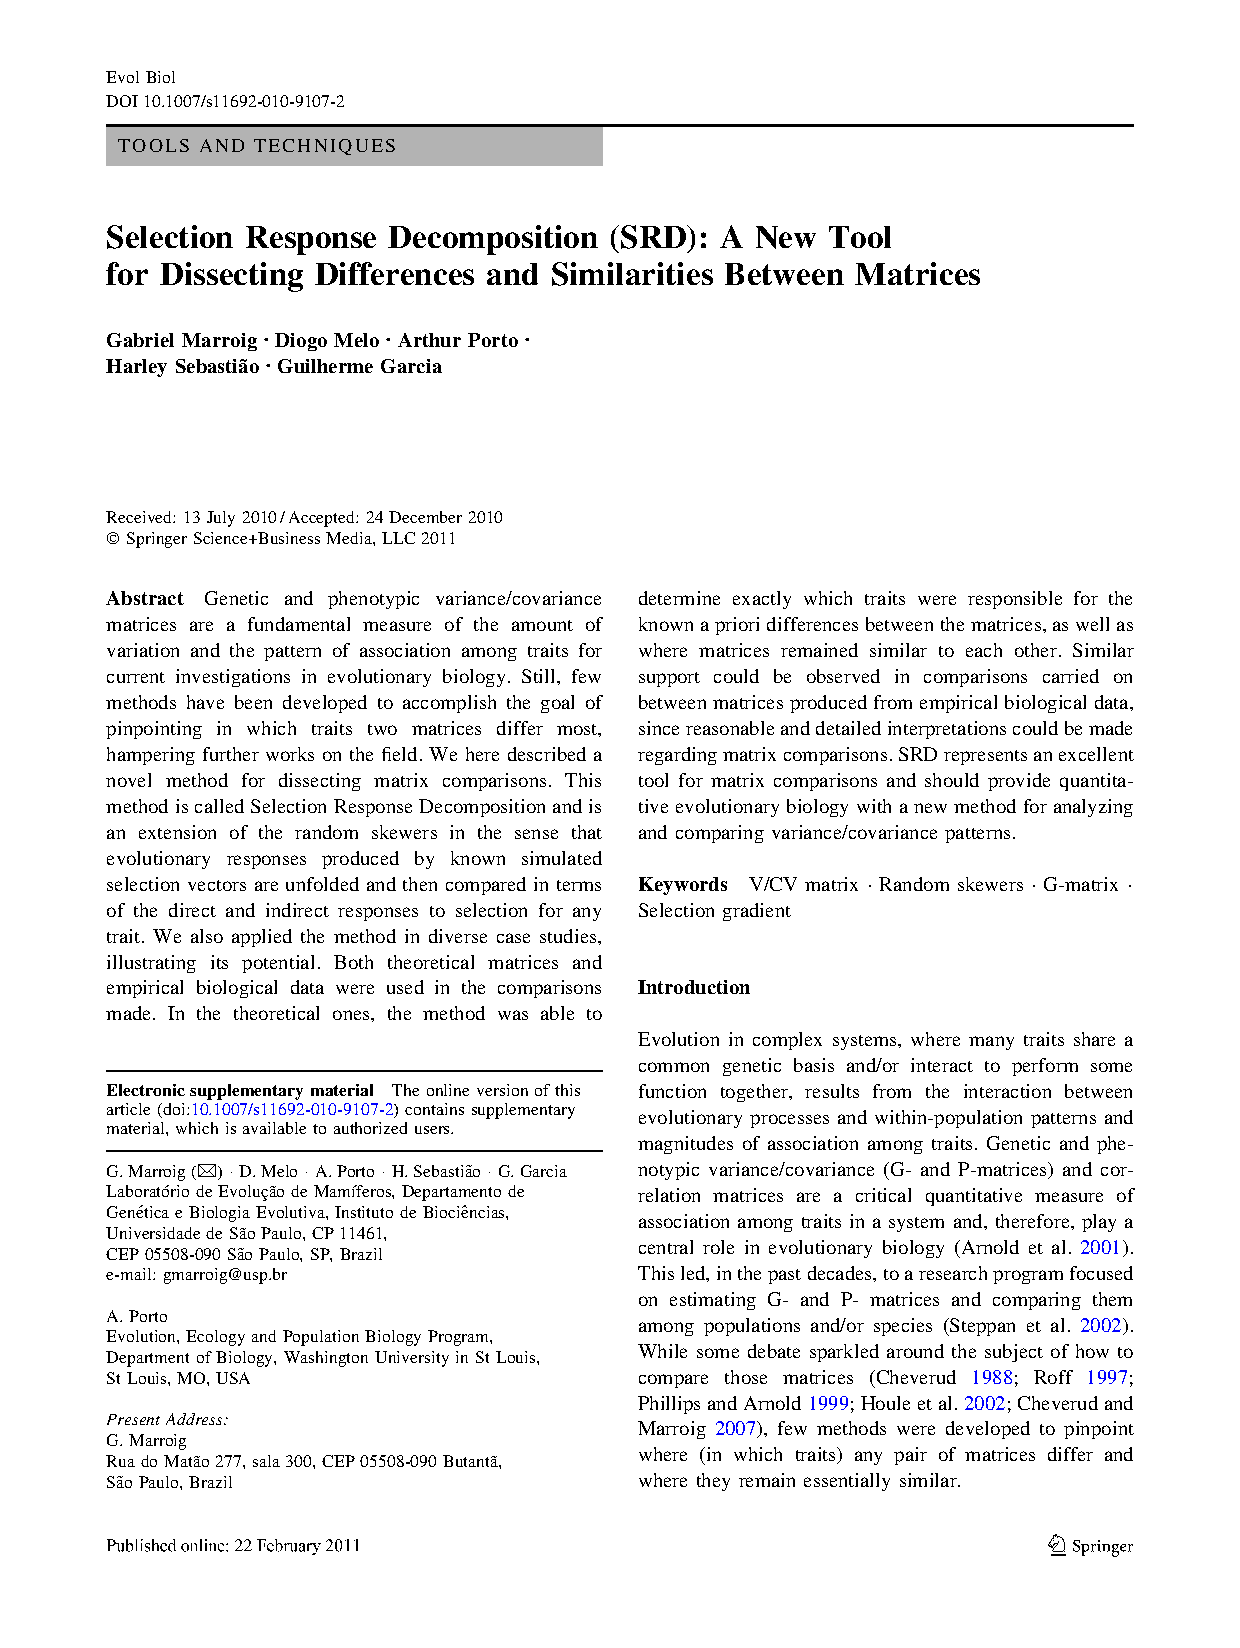
\includepdf[
            pages=-,
            width=189mm,
            height=267.3mm,
            offset=15pt 0pt,
            pagecommand={\pagestyle{plain}}
            ]{Appendix/Marroig2011.pdf}

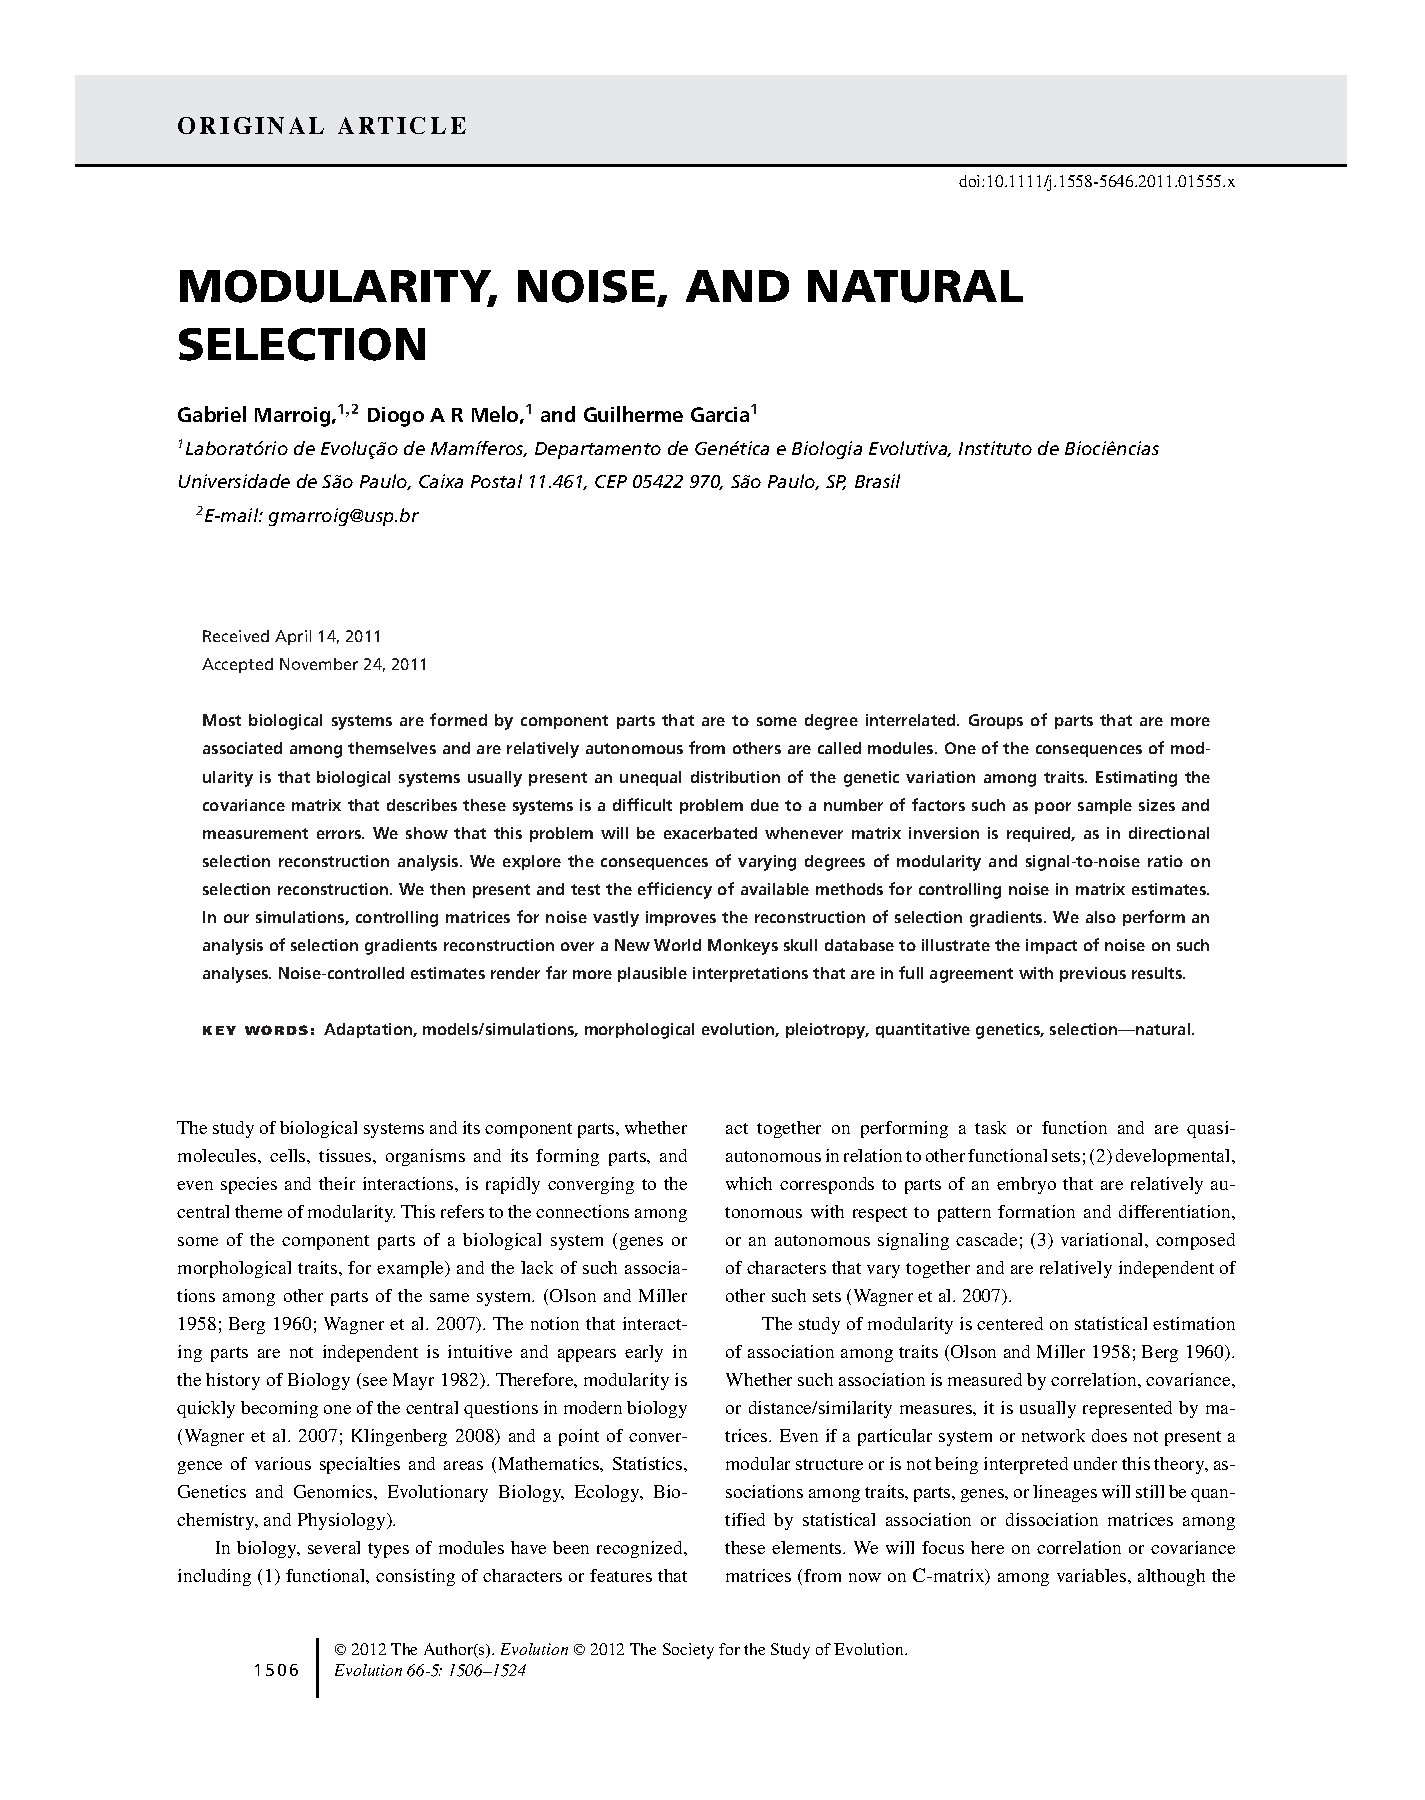
\includepdf[
            pages=-,
            width=189mm,
            height=267.3mm,
            offset=15pt 0pt,
            pagecommand={\pagestyle{plain}}
            ]{Appendix/Marroig2012.pdf}

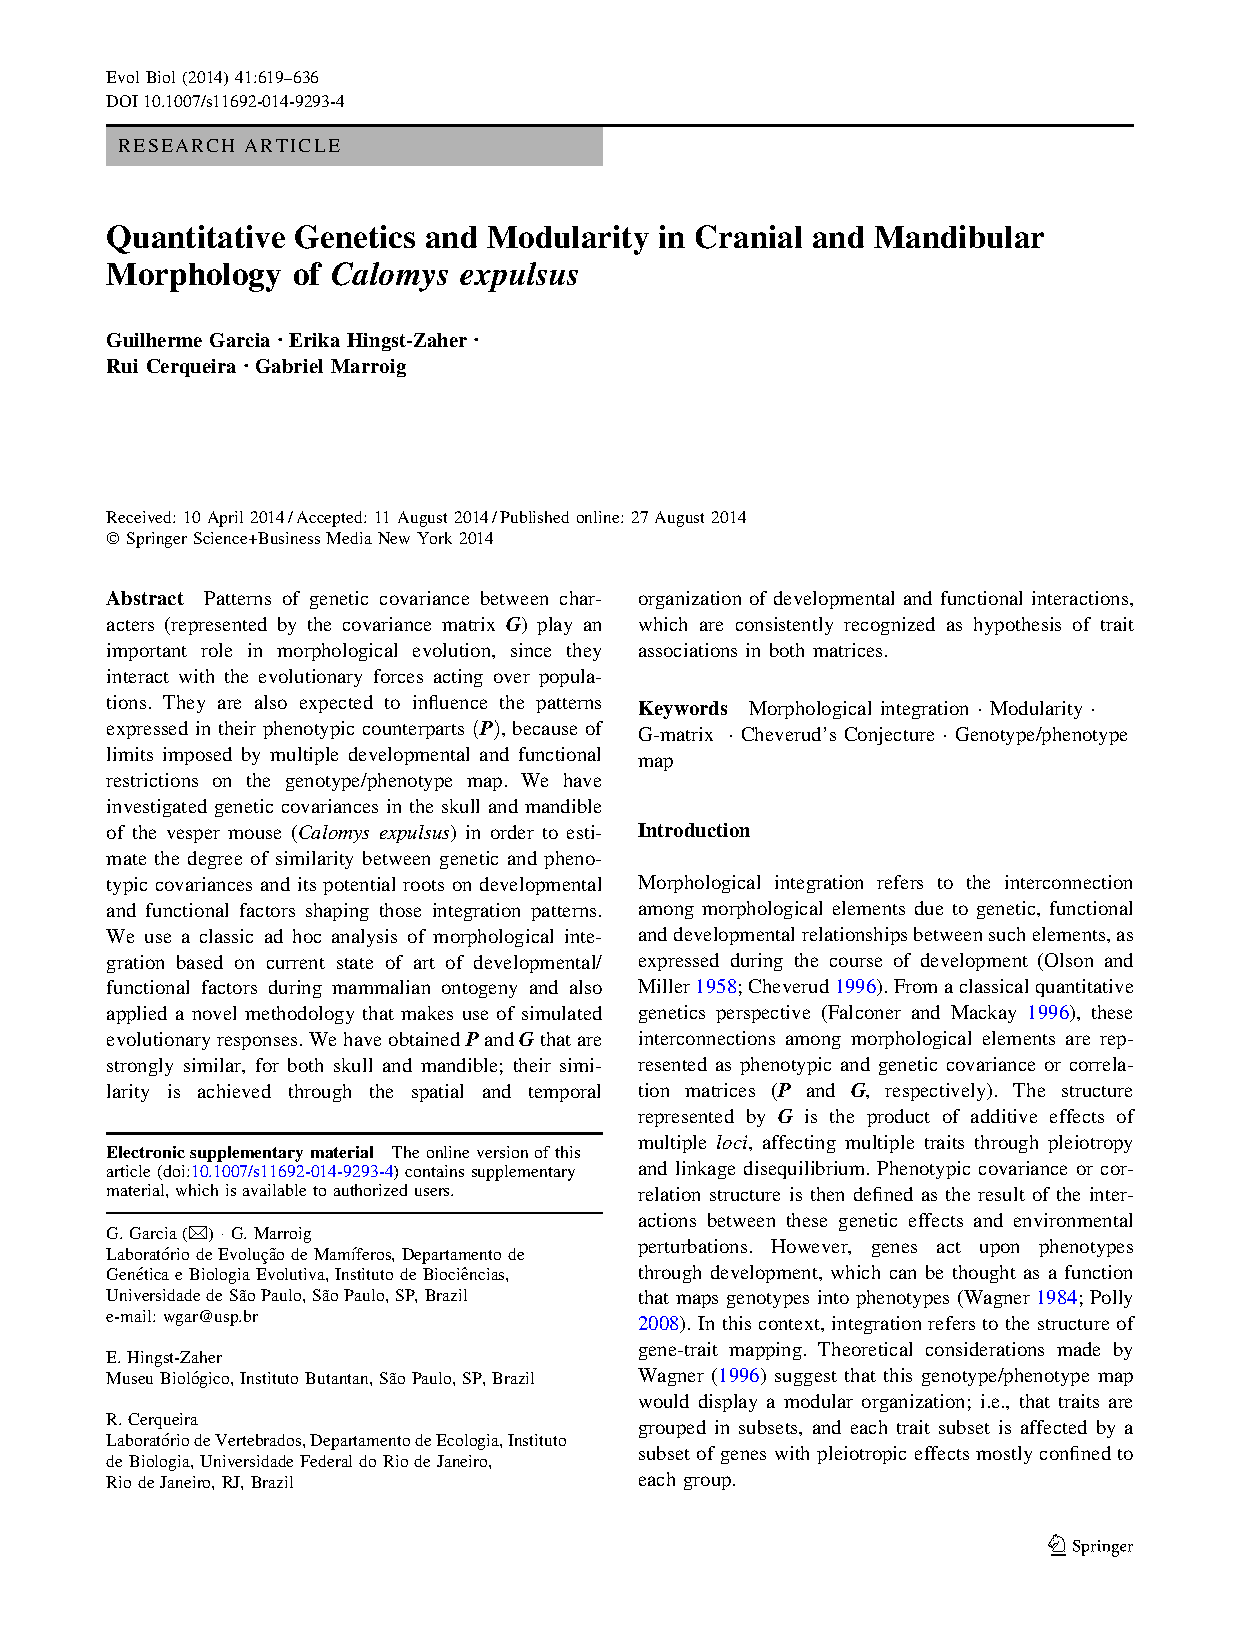
\includepdf[
            pages=-,
            width=189mm,
            height=267.3mm,
            offset=15pt 0pt,
            pagecommand={\pagestyle{plain}}            
            ]{Appendix/Garcia2014.pdf}

\end{document}
